% Copyright 2022 Haute école d'ingénierie et d'architecture de Fribourg
%
% Licensed under the Apache License, Version 2.0 (the "License");
% you may not use this file except in compliance with the License.
% You may obtain a copy of the License at
%
% http://www.apache.org/licenses/LICENSE-2.0
%
% Unless required by applicable law or agreed to in writing, software
% distributed under the License is distributed on an "AS IS" BASIS,
% WITHOUT WARRANTIES OR CONDITIONS OF ANY KIND, either express or implied.
% See the License for the specific language governing permissions and
% limitations under the License.

% =============================================================================
% | HES-SO//Master - Thesis project report template                           |
% |                                                                           |
% | Originally based on the EPFL template, with many adjustments             |
% =============================================================================

% Document settings
\documentclass[a4paper,11pt,fleqn]{book}
\usepackage[utf8]{inputenc}
\usepackage[T1]{fontenc} 
\usepackage[french]{babel}



% -----------------------------------------------------------------------------
% Preamble
% -----------------------------------------------------------------------------
% =============================================================================
% | Thesis metadata                                                           |
% =============================================================================

% Thesis info
\newcommand{\ThesisTitle}{Prédiction des propriétés chimiques par machine learning}
\newcommand{\ThesisSubject}{}
\newcommand{\Orientation}{Information and communication systems (ICS) }
\newcommand{\Keywords}{}
\newcommand{\Keywordsfr}{}
\newcommand{\projectVersion}{v1.1}
\newcommand{\cdcVersion}{v1.0}

% Author
\newcommand{\AuthorFirstName}{Simon }
\newcommand{\AuthorLastName}{Barras}
\newcommand{\AuthorEmail}{simon.barrasl@edu.hefr.ch}
\newcommand{\Author}{\AuthorFirstName \AuthorLastName}

% Advisor
\newcommand{\AdvisorFirstName}{Beat }
\newcommand{\AdvisorLastName}{Wolf}
\newcommand{\AdvisorSchool}{HEIA-FR}
\newcommand{\Advisor}{Prof. \AdvisorFirstName \AdvisorLastName}
\newcommand{\AdvisorTwoFirstName}{Jonathan }
\newcommand{\AdvisorTwoLastName}{Donzallaz}
\newcommand{\AdvisorTwoSchool}{HEIA-FR}
\newcommand{\AdvisorTwo}{Assis. \AdvisorTwoFirstName \AdvisorTwoLastName}

% Main expert - TODO: suppress?
\newcommand{\ExpertFirstName}{[FirstName]}
\newcommand{\ExpertLastName}{[LastName]}
\newcommand{\Expert}{\ExpertFirstName \ExpertLastName}
\newcommand{\ExpertLab}{[Lab/Company]}

% Mendant
\newcommand{\MendantInstitut}{Inst. ChemTech}
\newcommand{\MendantOneFirstName}{Roger }
\newcommand{\MendantOneLastName}{Marti}
\newcommand{\MendantOneSchool}{HEIA-FR}
\newcommand{\MendantOne}{Prof. \MendantOneFirstName \MendantOneLastName}
\newcommand{\MendantTwoFirstName}{Florence }
\newcommand{\MendantTwoLastName}{Yerly}
\newcommand{\MendantTwoSchool}{HEIA-FR}
\newcommand{\MendantTwo}{Prof. \MendantTwoFirstName \MendantTwoLastName}

% Place (for date and place)
\newcommand{\Date}{\today}
\newcommand{\Place}{Fribourg}
         % your project data
% ==================
% Template settings
% ==================

% General tools
% -------------
\usepackage{etoolbox}
\usepackage{listings}

% Page style
% ----------
\usepackage[margin=3cm, left=3.5cm, right=3.5cm, twoside=false]{geometry}
\usepackage{fancyhdr}
\setlength{\headheight}{14pt}
\renewcommand{\sectionmark}[1]{\markright{\thesection\ #1}}
\pagestyle{fancy}

% Standard pages (inside chapters)
\fancyhf{}
\renewcommand{\headrulewidth}{0.4pt}
\renewcommand{\footrulewidth}{0.4pt}
\fancyhead[R]{\bfseries \nouppercase{\rightmark}}
\fancyhead[L]{\bfseries \nouppercase{\leftmark}}
\fancyfoot[L]{\Author \space - \ThesisTitle}
\fancyfoot[R]{\thepage}

% First page of chapters
\fancypagestyle{plain}{
	\fancyhf{}
	\renewcommand{\headrulewidth}{0pt}
	\fancyfoot[L]{\Author \space - \ThesisTitle}
	\fancyfoot[R]{\thepage}
}

% Imports for external PDFs
\fancypagestyle{addpagenumbersforpdfimports}{
	\fancyhead{}
	\renewcommand{\headrulewidth}{0pt}
	\fancyfoot{}
	\fancyfoot[R]{\thepage}
}

% Use empty style for page when clearing double pages
%\def\cleartoodd{%
%	\clearpage%
%	%\ifodd\value{page}\else\mbox{}\thispagestyle{empty}\newpage\fi%
%}

%\def\clearchap{%
%	\ifodd\value{page}\else\mbox{}\thispagestyle{empty}\fi%
%}

% \cleardoublepage replaced by \cleartoodd
%\let\origdoublepage\cleardoublepage
%\renewcommand{\cleardoublepage}{%
%	\cleartoodd%
%}

% Fonts
% -----

% Helvetica (Arial used in the MSE Word template)
\usepackage{helvet}

% Math
% ----
\usepackage{amsmath}  % better math

% Floats and figures
% ------------------
\usepackage{newfloat}          % floats
\usepackage[oneside]{caption}  % captions
\usepackage{subcaption}        % subcaptions
\usepackage[section]{placeins} % allows to put float barriers

% Float captions in italics, with label in margin
%\DeclareCaptionLabelFormat{title}{#1 #2}
%\DeclareCaptionLabelFormat{hangout}{\llap{#1 #2\hspace{5mm}}}
%\captionsetup{
%	format=hang,
%	labelformat=hangout,
%	singlelinecheck=false,
%	font={it}
%}

% Caption with source for figure
% TODO: improve this to use square brackets like the normal "caption"
\newcommand*{\captionsource}[3]{%
	\caption[{#1}]{%
		#2%
		
		\textbf{Source:} #3%
	}%
}

% Tables
% ------
\usepackage{booktabs} % much better tables
\usepackage{multirow} % allows to fuse rows
\usepackage{array}    % manipulate array
\usepackage{tabularx} % better tables

% Define new tabularx column types:
%  - R: streteched right aligned
%  - C: stretched centered
%  - N: left aligned, specified space
\newcolumntype{R}{>{\raggedleft\arraybackslash}X}%
\newcolumntype{C}{>{\centering\arraybackslash}X}%
\newcolumntype{N}[1]{>{\raggedleft\arraybackslash}p{#1}}

% Set row height multiplicator to provide more breathing space
\renewcommand{\arraystretch}{1.3} 

% Bibliography
% -------------------

% Use biber, with numeric style and no sorting (citation order)
\usepackage[
backend=biber,
style=numeric,
sorting=none,
bibencoding=auto
]{biblatex}
\addbibresource{bibliography.bib}


% Tables of contents, figures, tables and listings
% ------------------------------------------------
\usepackage{tocloft}
\newlistof{listing}{lol}{List of Listings}
\setcounter{tocdepth}{1} % Depth to 'section'
\setlength{\cftfigindent}{0pt}  % remove indentation from figures in lof
\setlength{\cftfignumwidth}{1cm}
\setlength{\cfttabindent}{0pt}  % remove indentation from tables in lot
\setlength{\cfttabnumwidth}{1cm}
\setlength{\cftlistingindent}{0pt}
\setlength{\cftlistingnumwidth}{1cm}

% Mini tables of contents
% -----------------------
\usepackage{minitoc}

% no "Contents" title
\mtcsettitle{minitoc}{Contents} 

% Layout
\setlength{\mtcindent}{-0.5em}
\mtcsetoffset{minitoc}{-1em}

% Spacing above and below table
\mtcsetfeature{minitoc}{before}{\vspace{0.5cm}}
\mtcsetfeature{minitoc}{after}{\vspace{-0.25cm}}
\renewcommand{\mtifont}{\sffamily\bfseries\large}

% Colors & graphics
% -----------------
\usepackage[table]{xcolor}    % colors
\usepackage[pdftex]{graphicx} % graphics importing
\graphicspath{{02-main/figures/}}
\definecolor{gray80}{gray}{0.80}


% Code and syntax highlighting
% ----------------------------
\usepackage[newfloat]{minted}   % code highlighting

% Typography
% ----------
\usepackage{csquotes}                    % paragraph indentation and spacing
\usepackage[defaultlines=3,all]{nowidow} % avoid widows and orphans
\usepackage{microtype}                   % typographic improvements
\usepackage{parskip}                     % No indent and auto-space between paragraphs
\usepackage[super]{nth}

\usepackage{paralist}
\usepackage{enumitem}
\setlist{after=\vspace{\baselineskip}}

% Section and chapters headings
% -----------------------------
\usepackage[explicit]{titlesec} % titles formatting
%\usepackage{titletoc} % titles formatting in ToC etc
%\usepackage{sectsty}  % sectioning commands

% -- Chapters --
% Remove "Chapter N" and use a sans-serif font

% Set layout lengths
\setlength{\headheight}{8mm}
\setlength{\footskip}{1.5cm}
\addtolength{\textheight}{-.5cm}

\titlespacing{\chapter}{-5mm}{-10mm}{3mm}
\titlespacing{\section}{-5mm}{3mm}{2mm}
\titlespacing{\subsection}{-5mm}{2mm}{2mm}
\titlespacing{\subsubsection}{-5mm}{2mm}{1mm}


%\titleformat{\chapter}[block]
%{\Huge}
%{\thechapter\hspace{12pt}\textcolor{gray80}{|}\hspace{12pt}}
%{0pt}
%{\Huge\bfseries}

\titleformat{\chapter}{\Huge\bfseries}{\llap{\thechapter\hspace{12pt}\textcolor{gray80}{|}}}{0mm}{%
	\hfill\begin{minipage}[t]{\dimexpr\textwidth}\raggedright#1\end{minipage}%
}
\titleformat{\section}{\Large\bfseries}{\llap{\thesection}}{0mm}{%
	\hfill\begin{minipage}[t]{\dimexpr\textwidth}\raggedright#1\end{minipage}%
}
\titleformat{\subsection}{\large \bfseries}{\llap{\thesubsection}}{0mm}{%
	\hfill\begin{minipage}[t]{\dimexpr\textwidth}\raggedright#1\end{minipage}%
}
\titleformat{\subsubsection}{\bfseries}{\llap{\thesubsubsection}}{0mm}{%
	\hfill\begin{minipage}[t]{\dimexpr\textwidth}\raggedright#1\end{minipage}%
}

% Misc
% ------
\usepackage{lipsum}    % filler text
\usepackage{blindtext} % random text
\usepackage{lscape}    % easy landscape pages
\usepackage{pdflscape} % landscape pages for PDFs

% Allow email typesetting
\newcommand{\email}[1]{%
	\href{mailto:#1}{\textit{#1}}%
}

% References
% -----------
\usepackage{url}

% pdf metadata
\usepackage[
	pdfauthor={\Author},
	pdftitle={\ThesisTitle},
	pdfsubject={\ThesisSubject},
	pdfkeywords={\Keywords}
	pdfduplex=DuplexFlipLongEdge]{hyperref}
		
% Hyperlinks
\hypersetup{
	colorlinks=true,
	linkcolor=black,
	citecolor=black,
	filecolor=black,
	urlcolor=black,
}
\providecommand*{\listingautorefname}{Listing}


% % Glossary
% % --------
%\usepackage[xindy,toc, nonumberlist]{glossaries}
\usepackage[acronym]{glossaries}
\makeglossaries
% Terms
% -----
% format:  \newglossaryentry{<label>}{<settings>}
% example: \newglossaryentry{computer}
%{
%	name=computer,
%	description={is a programmable machine that receives input,
%		stores and manipulates data, and provides
%		output in a useful format}
%}

\newglossaryentry{latex}
{
    name=latex,
    description={Is a markup language specially suited 
    for scientific documents}
}

% Acronyms
% --------
% format:  \newacronym{<label>}{<abbrv>}{<full>}
% example: \newacronym{lvm}{LVM}{Logical Volume Manager}
% plural:  \newacronym[longplural={Frames per Second}]{fpsLabel}{FPS}{Frame per Second}

    % template settings
% ===========================================
% = Codestyles for minted syntax highlighting
% ===========================================


% How to use (replace 'java' with language name):
% - code blocks:
%     \begin{javacode}
%     CODE
%     \end{javacode}
% - files:
%     full: \javafile{PATH}
%     extract: \javafile[startline=x, endline=y]{PATH}

% c#
\newminted{csharp}{frame=single, framesep=6pt, breaklines=true, fontsize=\scriptsize}
\newmintedfile{csharp}{frame=single, framesep=6pt, breaklines=true, 
fontsize=\scriptsize}

% Java
\newminted{java}{frame=single, framesep=6pt, breaklines=true, fontsize=\scriptsize}
\newmintedfile{java}{frame=single, framesep=6pt, breaklines=true, 
fontsize=\scriptsize}

% JavaScript
\newminted{js}{frame=single, framesep=6pt, breaklines=true, fontsize=\scriptsize}
\newmintedfile{js}{frame=single, framesep=6pt, breaklines=true, fontsize=\scriptsize}

% Scala
\newminted{scala}{frame=single, framesep=6pt, breaklines=true, fontsize=\scriptsize}
\newmintedfile{scala}{frame=single, framesep=6pt, breaklines=true, 
	fontsize=\scriptsize}

% Clojure
\newminted{clojure}{frame=single, framesep=6pt, breaklines=true, fontsize=\scriptsize}
\newmintedfile{clojure}{frame=single, framesep=6pt, breaklines=true, 
	fontsize=\scriptsize}

% Python
\newminted{python}{frame=single, framesep=6pt, breaklines=true, fontsize=\scriptsize}
\newmintedfile{python}{frame=single, framesep=6pt, breaklines=true, fontsize=\scriptsize}

% Sql
\newminted{sql}{frame=single, framesep=6pt, breaklines=true, fontsize=\scriptsize}
\newmintedfile{sql}{frame=single, framesep=6pt, breaklines=true, fontsize=\scriptsize}

% Json
\newminted{json}{frame=single, framesep=6pt, breaklines=true, fontsize=\scriptsize}
\newmintedfile{json}{frame=single, framesep=6pt, breaklines=true, 
	fontsize=\scriptsize}

% Yaml
\newminted{yaml}{frame=single, framesep=6pt, breaklines=true, 
fontsize=\scriptsize}
\newmintedfile{yaml}{frame=single, framesep=6pt, breaklines=true, 
	fontsize=\scriptsize}

% Plain text
\newminted{text}{frame=single, framesep=6pt, breaklines=true, breakanywhere, fontsize=\scriptsize}
\newmintedfile{text}{frame=single, framesep=6pt, breaklines=true, breakanywhere, fontsize=\scriptsize}       % code styles for minted
% ========================
% = TODO: Document
% ========================

% Marc's font stack
\usepackage{cmbright}       % Sans serif
\usepackage{sourcecodepro}  % Monospace
\usepackage{float}
\renewcommand{\familydefault}{\sfdefault}
  % your custom packages etc

% Glossary
% --------

% \usepackage[toc]{glossaries}
% \makeglossaries
% % Terms
% -----
% format:  \newglossaryentry{<label>}{<settings>}
% example: \newglossaryentry{computer}
%{
%	name=computer,
%	description={is a programmable machine that receives input,
%		stores and manipulates data, and provides
%		output in a useful format}
%}

\newglossaryentry{latex}
{
    name=latex,
    description={Is a markup language specially suited 
    for scientific documents}
}

% Acronyms
% --------
% format:  \newacronym{<label>}{<abbrv>}{<full>}
% example: \newacronym{lvm}{LVM}{Logical Volume Manager}
% plural:  \newacronym[longplural={Frames per Second}]{fpsLabel}{FPS}{Frame per Second}


\begin{document}


% -----------------------------------------------------------------------------
% Front matter
% -----------------------------------------------------------------------------
\frontmatter

\dominitoc

% ==========================================================================
% = HES-SO Master thesis title page (modeled after Word template, 2016-2017)
% ==========================================================================

\begin{titlepage}
\newgeometry{margin=2cm}
{\fontfamily{phv}\fontseries{mc}\selectfont
    \begin{center}
	    
\includegraphics[width=0.95\textwidth]{img/heiafr_logo}
		~\\[1.5cm]
		% Title
		{
			\Huge
			PS5 - \ThesisTitle\\Rapport de projet \\[0.5cm]
			\large Informatique et Système de Communication (ISC), 2022-2023\\[2cm]
		}
		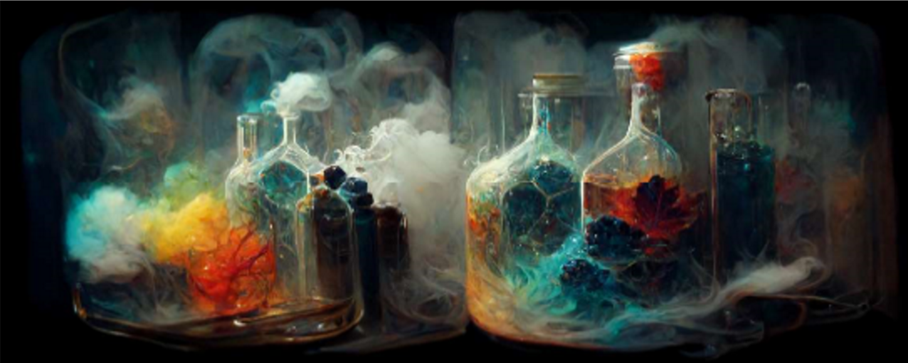
\includegraphics[width=0.8\textwidth]{img/logo.png}
		~\\[2cm]
		% Info
		{
			\begin{center}
			\begin{tabularx}{\textwidth} { %tableau pour créer 2 colonnes 
				>{\raggedright\arraybackslash}X 
				>{\raggedright\arraybackslash}X  }
					 \textbf{Etudiant} & \Author\\
					 & \\
					 \textbf{Enseignants responsables} & \Advisor \space - \AdvisorSchool \\ & \AdvisorTwo \space - \AdvisorTwoSchool \\
					 & \\
					 \textbf{Mendant} & \MendantInstitut \\ & \MendantOne \space - \MendantOneSchool \\ & \MendantTwo \space - \MendantTwoSchool\\
			\end{tabularx}
			\end{center}
			~\\[1.5cm]
		}
%		{
%			\large
%			External expert: \\
%			\Expert
%		}

        % {
        % Le code de ce projet est disponible en open source avec l'accord de tous ses
        % participants.
        % }
		\vfill
		
		 
		
		% Bottom of the page
	    {\projectVersion}\\
		{\large \Place, HEIA-FR, \Date}
		
	\end{center}
}
\restoregeometry
\end{titlepage}






% Page for student info and signatures
% \cleardoublepage
% \chapter*{Information about this report}

\vspace{\fill}

\textbf{Contact information}

\begin{tabularx}{\textwidth}{N{2.5cm}X}
	Author:	 & \AuthorFirstName \AuthorLastName \\
	& MSE Student \\
	& HES-SO//Master \\
	& Switzerland \\
	Email: & \email{\AuthorEmail}
\end{tabularx}

\vspace{\fill}

\textbf{Declaration of honor}

{\renewcommand{\arraystretch}{2}
\begin{tabularx}{\textwidth}{N{2.5cm}X}
	& I, undersigned, \Author, hereby declare that the work submitted is 
	the result of a personal work. I certify that I have not resorted to 
	plagiarism or other forms of fraud. All sources of information used and the 
	author quotes were clearly mentioned. \\
	Place, date: & \underline{\hspace{7cm}} \\ 
	Signature: & \underline{\hspace{7cm}}
\end{tabularx}
}

\vspace{\fill}

%\textbf{Validation}

%Accepted by the HES-SO//Master (Switzerland, Lausanne) on a proposal from:
Accepté par la HES SO//Master (Suisse, Lausanne) sur proposition de

\vspace{0.5cm}

\Advisor %, Thesis project advisor

%\Expert, \ExpertLab, Main expert

\vspace{1cm}

Lieu, date: \underline{\hspace{8cm}}

\vspace{3cm}

{ \renewcommand{\arraystretch}{1.5}
\begin{tabularx}{\textwidth}{X X}
	\Advisor  & \Dean\\ 
	Advisor   & Dean, HES-SO//Master\\
\end{tabularx}
}

% Acknowledgments (your dedication etc)
% \cleardoublepage
% \chapter*{Acknowledgments}
\markboth{Acknowledgements}{Acknowledgements}
\addcontentsline{toc}{chapter}{Acknowledgements}

% -- Your text goes here --
\lipsum[1-2]
 


% Preface (to be written by someone else)
% \cleardoublepage
% \chapter*{Preface}
\markboth{Preface}{Preface}
\addcontentsline{toc}{chapter}{Preface}
% put your text here
A preface is not mandatory. It would typically be written by some other person (eg your thesis director).

\lipsum[1-2]

\bigskip
 
\noindent\textit{Lausanne, 12 Mars 2011}
\hfill T.~D.


% French + English abstracts
%\cleardoublepage
%% English abstract
\chapter*{Abstract}
%\markboth{Abstract}{Abstract}
\addcontentsline{toc}{chapter}{Abstract} % adds an entry to the table of contents

\vskip0.5cm
\textbf{Key words: } 
\Keywords


% French abstract
% \cleardoublepage
% \begin{otherlanguage}{french}
% \chapter*{Résumé}
% %\markboth{Résumé}{Résumé}

% \lipsum[1-2]

% \vskip0.5cm
% \textbf{Mots clés:} 
% \Keywordsfr
% \end{otherlanguage}



% Table of contents
\phantomsection
\chapter{Historique des versions}
\label{chap:versions}

\begin{tabular}{|m{0.15\textwidth}|m{0.7\textwidth}|m{0.15\textwidth}|} 
 \hline
 \textbf{Version} & \textbf{Changements} & \textbf{Date} \\ [0.5ex] 
 \hline
 0.1 & Document créé sur la base du cahier des charges et les chapitres introduction et reproduction des résultats & 15.10.2022  \\ 
 \hline
 0.2 & Nouvelle structure et reformulation du chapitre sur la reproduction des résultats qui a été déplacé au point 4.1 & 27.11.2022  \\ 
 \hline
 0.3 & Ajout de la première partie du chapitre analyse et correction du chapitre 4.1 par rapport aux illustrations & 07.12.2022  \\ 
 \hline
 0.4 & Fin de la partie analyse et commencement de la partie conception & 17.01.2023  \\ 
 \hline
 1.0 & Première rédaction complète du rapport & 01.02.2023  \\ 
 \hline
 1.1 & Correction des fautes d'orthographe et réécriture de certains chapitres & 02.02.2023  \\ 
 \hline
\end{tabular}
\addcontentsline{toc}{chapter}{Table des matières}
\setcounter{tocdepth}{2}
\tableofcontents

% List of tables
% \cleardoublepage
% \phantomsection
% \addcontentsline{toc}{chapter}{Liste des tables}
% \listoftables

% List of listings
% \cleardoublepage
% \phantomsection
% \addcontentsline{toc}{chapter}{List of Listings}
% \listoflistings

% Restore paragraphs
\setlength{\parskip}{1em}

% Bold fonts for sections in minitoc
\renewcommand{\cftsecfont}{\sffamily\bfseries}
\renewcommand{\cftsecleader}{\sffamily\bfseries\cftdotfill{\cftdotsep}}
\renewcommand{\cftsecpagefont}{\sffamily\bfseries}


% -----------------------------------------------------------------------------
% Main matter
% -----------------------------------------------------------------------------
\mainmatter

% Chapters
\setcounter{mtc}{4} % Help minitoc skip the front matter chapters
\chapter{Introduction}
\label{chap:introduction}
% -----------------------------------------------------------------------------

Ce projet a pour but d'aider l'institut ChemTech de la \acrshort{heia-fr} pour les recherches futures utilisant des liquides ioniques.
Ces liquides ioniques sont des éléments qui sont beaucoup utilisés en chimie.
Ils permettent notamment de stocker de l'énergie mais disposent aussi de nombreuses autres applications.

Les liaisons ioniques s'obtiennent par l'attraction de deux ions de charge opposée.
Les ions de charges positives et négatives sont respectivement appelés : cation et anion.
Généralement, les cations sont métalliques tandis que les anions ne le sont pas.
Un ion est composé d'un ou plusieurs atomes chargés électriquement.

Les possibilités de liaisons sont probablement infinies et leurs propriétés diffèrent pour chaque composition.
Dans notre cas, la particularité qui nous intéresse est le point d'ébullition.
Si on voulait obtenir cette information par expérience, il faudrait compter en jour le temps et les ressources consommées seraient importantes.
L'objectif de ce travail de semestre est d'estimer la température d'ébullition d'un liquide ionique afin de concentrer le temps et les ressources de l'institut ChemTech de la \acrshort{heia-fr} sur des liaisons validées par l'outil au préalable.

Ce travail sera utilisé comme outil de base pour un projet visant à stocker ou récupérer de l'énergie dans les phases de changements d'états d'un liquide ionique.
Le but est d'y insérer en entrée le \acrfull{smiles} de l'anion et du cation et d'en obtenir la température estimée.

L'écriture \acrshort{smiles} est utilisée en chimie pour décrire des molécules.
Cette écriture permet de reconstruire le modèle 3D ou 2D comme ci-dessous :
\begin{center}
   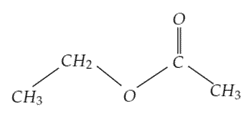
\includegraphics[height=20mm]{img/smiles_example.png}
   \captionof{figure}{Exemple de \acrshort{smiles}}
\end{center}

 
Il existe une librairie python qui permet de récupérer les informations issues d'un \acrshort{smiles}.

Ce projet a déjà été amorcé par Mme Yerly et Denis Marti, collaborateur effectuant son service civil à la \acrshort{heia-fr}.
Ils ont réussi à reproduire les résultats obtenus dans une étude\cite{WANG2021432} à l'aide de la base de données fournie par cette dernière et vérifier par la base de données de l'école.
Ce modèle était basé sur l'algorithme \acrfull{svm}.

Ces algorithmes ont besoin de données d'entrées et de cibles.
leur but sera de faire le lien entre les différents paramètres insérés et la cible la plus probable.

Dans un second temps, on pourrait aussi imaginer améliorer l'outil en rajoutant une surcouche qui déterminera le meilleur liquide ionique pour un objectif donné ou la possibilité de prédire d'autres propriétés.


\section{Objectifs}

Les Objectifs de ce projet sont découpés en deux catégories par niveau d'importance.


Les objectifs principaux consistent à reproduire les résultats de l'étude de Mme Yerly et de l'étudiant en master de mathématiques ainsi que regrouper et normaliser toutes les données nécessaires pour créer des modèles de \acrlong{ml}.
Le dernier objectif principale est le plus long et le plus intéressants car il faut créer un nouveau modèle à l'aide de l'écriture \acrshort{smiles}.


Les objectifs secondaires sont des améliorations qui pourraient être faites aux objectifs principaux.
Par exemple, nous avons la recherches de nouvelles données, le test de plusieurs algorithmes de \acrlong{ml} ou encore l'amélioration de l'\acrlong{ux}.
En effet, les interactions utilisateurs seront très sommaires et il y a beaucoup de chose envisageable comme une \acrshort{api}, un \acrshort{cli} ou une interface graphique.


\section{Activités}

Les activités sont découpées en 3 milestones. La première représente la phase de reproduction des résultats de l'étude de Mme Yerly et la mise en places des données normalisées.
La deuxième milestone représente la phase de création d'un nouveau modèle à l'aide de l'écriture \acrshort{smiles} et la troisième milestone représente la phase d'amélioration de l'outil.

Pour organiser le travail, j'utilise GitLab et le système d'épiques pour représenter le diagramme de Gantt.
Les avantages de ce systèm est que tout est centralisé à un seul endroit et le code peut être directement lié aux tâches, cependant la gestion de projet de GitLab a quelques désavantages comme par exemple, le diagramme de Gantt n'est pas très pratique à utiliser.


\chapter{Etat de l'art}
\label{chap:stateoftheart}

Ce projet ne part pas de zéro.
En effet, Mme Yerly est une enseignante de mathématiques à la \acrshort{heia-fr} qui a proposé un modèle de \acrlong{ml} pour prédire le point d'ébullition d'un liquide ionique.
Elle a réalisé ce projet\cite{IL_SVM_report} avec l'aide de M Marti en se basant sur une étude d'un chercheur qui s'appelle Wang\cite{WANG2021432}.

Le modèle qu'ils ont réalisé obtient des résultats satisfaisants mais il est limité par les données qu'ils ont utilisées.
En effet, ce modèle se base seulement sur la présence ou non de certaines molécules dans la composition du liquide ionique.

% -----------------------------------------------------------------------------
\section{Analyse}
\label{sec:stateoftheart:analysis}
L'idée de ce projet est de déterminer le point de fusion d'un liquide ionique à partir de la présence ou non de molécules.
L'étude de bases\cite{WANG2021432} fournie des données et certaines d'entre elles ont été ajoutées par la HEIAFR.
Le but est de préprocesser ces données avec l'algorithme de normalisation \acrshort{minimax} puis de faire une régression avec \acrshort{svm}.

\subsection{Données}
Les données de base sont fournies dans un tableau excel\cite{SVM_data} mais elles se trouvent aussi dans le nouveau fichier créé pour ce projet\cite{New_data}.
Le dataset contient 102 colonnes dont deux qui sont inutiles car ce sont les noms des anions et des cations.
Les 99 features ont des valeurs entre 0 et 30 et représentent la présence ou non d'une molécule dans la composition du liquide ionique.
Le dataset d'entraînement contient 600 lignes qui sont toutes complètes et aucune ligne n'est dupliquée.
La valeur cible est la colonne \texttt{Exp (K)} qui représente le point de fusion en degrés Kelvin.
La moyenne des points de fusions est de 322,29 K et la médiane de 318,5 K.
Les valeurs se situent entre 177,15 et 550,15 Kelvin ce qui nous fait un écart-type de 54, 37 K.
Voici l'historgramme des points de fusion selon pandas-profiling\cite{pp_old}:
\begin{center}
    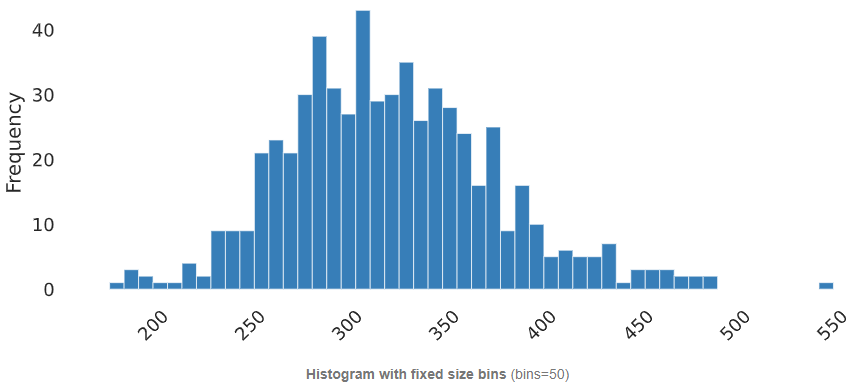
\includegraphics[width=140mm]{img/histogram_exp_old_pp.png  }
    \captionof{figure}{Histrogramme fourni par pandas profiling des points de fusions des données de base}
\end{center}

\subsection{Préprocessing}
Le preprocessing des données est important car il permet de les mettre en forme ces dernières dans un intervalle défini.
Ceci permet d'éviter un problème de poids inégale entre les features dus à la grandeur des distances.
Il existe plusieur méthodes de scalling et elles sont presque toutes utilisables avec scikit-learn\cite{scikit-learn}.
L'algorithme de normalisation utilisé dans ce cas est \acrshort{minimax} et il est plus détaillé dans le chapitre \ref{analyse:ml:normalisation:minimax}.

\subsection{Régression}
La régression consiste à adapter une fonction afin de prédire une valeur numérique.
Dans ce projet, le but est de trouver les températures de fusion des liquides ioniques à partir de la présence ou non de molécules.
La première version de ce projet utilise l'algorithme \acrfull{svm} de la libraire LibSVM\cite{libsvm_doc}.
Plus précisément, il utilise une variante appelée \acrshort{nusvr} qui est détaillée dans le chapitre \ref{analyse:ml:algorithme:svm}.
Le but est de reproduire les résultats en utilisant la librairie scikit-learn\cite{scikit-learn} qui est une librairie python qui permet de faire du \acrlong{ml}.


% -----------------------------------------------------------------------------
\section{Conception}
Lors de l'obtention des résultats de la part de Mme Yerly et M Marti, ils ont du emprunter un certain cheminement.
Le but est de reproduire fidellement ce cheminement mais avec le nouveau fichier\cite{New_data} et \acrlong{sklearn}\cite{scikit-learn}.

\subsection{Préprocessing}
Le preprocessing utilisé est l'algorithme \acrshort{minimax} qui permet de normaliser les données.
Il est appliqué sur les features et la valeur cible.
Il ne faudra donc pas oublier de dénormaliser les valeurs prédites.

\subsection{Régression}
\label{sec:conception_regression}
Mme Yerly er M Marti ont utilisé la librairie libsvm\cite{libsvm_doc} pour faire la régression.
Pour ce projet, il faut utiliser la librairie scikit-learn\cite{scikit-learn} car elle permte de changer plus facilement d'algorithme et propose d'autres fonctionalitées.
Ceci ne devrait pas poser problème car elle utilise la librairie libsvm\cite{libsvm_doc} pour faire les \acrlong{svm}.

Une fois que la reproduction est faite, il est intéressant de tester d'autres algorithmes pour voir si les résultats sont meilleurs.

\subsubsection{Les hyper paramètres}
Les hyper paramètres optimaux sont donnés dans le rapport\cite{IL_SVM_report} de Mme Yerly et M Marti ets ont les suivants: texttt{-s 4 -t 2 -g 0.0272 -c 65}.
Si on traduit ces paramètres pour scikit-learn nous obtenons le tableau suivant:
\begin{table}[ht]
    \centering
    \begin{tabular}{|l|l|}
    \hline
    \textbf{LibSVM} & \textbf{Scikit-learn} \\ \hline
    -s 4            & Algorithme \acrshort{nusvr}      \\ \hline
    -t 2            & Regression \acrshort{nusvr}    \\ \hline
    -g 0.0272       & gamma=0.0272          \\ \hline
    -c 65           & C=65                  \\ \hline
    \end{tabular}
    \caption{Traduction des hyper paramètres de libsvm vers scikit-learn}
\end{table}


% -----------------------------------------------------------------------------
\section{Implémentation}
La reproduction des résultats s'obtient assez facilement avec la libraire scikit-learn\cite{scikit-learn}.
Il faut lire les données, les modifier et entrainer le modèle avec.

Pour reproduire les résultats, il suffit d'utiliser le script\cite{fusion_perdictor} de la manière suivante:
\begin{lstlisting}[language=bash]
    python fusion_predictor.py -ob -m minmax -a nusvr train
\end{lstlisting}
Il construira le dataset avec les données de bases et entraînera le modèles de l'étude de Mme Yerly et M Marti.

Le paramèptre -o permet de lire les anciennes données.
-n et -a permettent de choisir le scaler et l'algorithme.
Le paramètre -b indique si les targets doivent normalisées.
Le dernier paramètre indique l'action que nous voulons faire.

\subsection{Lecture des données}
Les données sont stockées dans un ficher Excel qui peut être lu avec la librairie \acrfull{pandas}.
Pour lire les données il ne faut pas oublier d'enlever les lignes et les colonnes non numériques.

\subsection{Préparation des données}
Les données doivent être prépocesser avec \acrshort{minimax} de scikit-learn.
Pour avoir les mêmes résultats que Mme Yerly et M Marti, il faut normaliser les features et la target.
Comme les données cibles prédites seront entre 0 et 1, il ne faudra pas oublier des dénormaliser avant de calculer quelquonques métriques.

\subsection{Entrainement du modèle}
L'entrainement du modèle se fait simplement avec sckiti-learn et les paramètres défini dans le chapitre \ref{sec:conception_regression}.


% -----------------------------------------------------------------------------
\section{Résultats}
Mme Yerly et M Marti ont entrainé leur modèle pour avoir le meilleure résultat prossible.
Voici une comparaison des résultats obtenus avec les données d'entraînement et de test:

\begin{table}[ht]
    \centering
    \begin{tabular}{l|cc|cc|}
    \cline{2-5}
    \multicolumn{1}{c|}{}              & \multicolumn{2}{c|}{\textbf{Etude}}                            & \multicolumn{2}{c|}{\textbf{Reproduction}}                     \\
    \multicolumn{1}{c|}{\textbf{}}     & \multicolumn{1}{c|}{\textbf{Training set}} & \textbf{Test set} & \multicolumn{1}{c|}{\textbf{Training set}} & \textbf{Test set} \\ \hline
    \multicolumn{1}{|l|}{\textbf{\acrshort{mse}}} & \multicolumn{1}{c|}{386.85}                & 515.47            & \multicolumn{1}{c|}{386.97}                & 516.12            \\ \hline
    \multicolumn{1}{|l|}{\textbf{\acrshort{mae}}} & \multicolumn{1}{c|}{?}                     & ?                 & \multicolumn{1}{c|}{13.18}                 & 18.1              \\ \hline
    \multicolumn{1}{|l|}{\textbf{\acrshort{me}}}  & \multicolumn{1}{c|}{?}                     & ?                 & \multicolumn{1}{c|}{103.1}                 & 69.78             \\ \hline
    \multicolumn{1}{|l|}{\textbf{$R^2$}}   & \multicolumn{1}{c|}{87\%}                  & 82.5\%            & \multicolumn{1}{c|}{86.89\%}               & 81.79\%           \\ \hline
    \end{tabular}%
    \caption{Comparaison des résultats entre l'étude et la reproduction}
\end{table}

La légère différence n'est pas significative.
Si on affiche les données prédites et les données réelles, on obtient le graphique suivant:

\begin{figure}[ht]
    \centering
    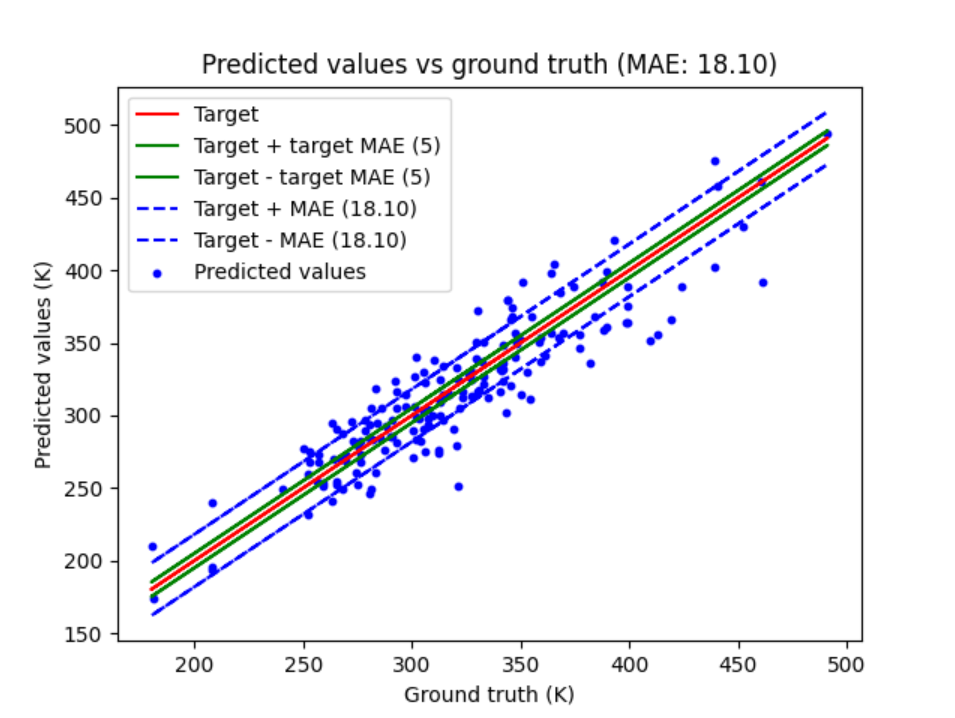
\includegraphics[width=0.8\columnwidth]{img/graphic_reproduction_result.png}
    \caption{Comparaison des données prédites et des données réelles pour la reproduction}
\end{figure}

L'objectif de l'institut est de prédire des données avec un \acrlong{mae} de cinq.
Le modèle actuel est très loin de cet objectif.

\subsection{D'autres algorithmes}
Scikit-learn permet de facilement changer d'algorithme.
Pour lancer la reproduction avec un autre algorithme, il faut modifier le paramètre -a.
Voici les résultats obtenus avec les autres algorithmes:

\begin{table}[ht]
    \centering
    \begin{tabular}{l|c|c|c|c|}
    \cline{2-5}
    \multicolumn{1}{c|}{\textbf{}}     & \textbf{nuSVR} & \textbf{SVR} & \textbf{Gradient boosting} & \textbf{Random forest} \\ \hline
    \multicolumn{1}{|l|}{\textbf{\acrshort{mse}}} & 516.12         & 870.3        & 1148.9                     & 959.36                 \\ \hline
    \multicolumn{1}{|l|}{\textbf{\acrshort{mae}}} & 18.1           & 23.91        & 26.17                      & 22.67                  \\ \hline
    \multicolumn{1}{|l|}{\textbf{\acrshort{me}}}  & 69.78          & 86           & 105.95                     & 116.45                 \\ \hline
    \multicolumn{1}{|l|}{\textbf{$R^2$}}   & 81.79\%        & 69.29\%      & 59.47\%                    & 66.15\%                \\ \hline
    \end{tabular}%
    \caption{Résultats des autres algorithmes avec les données de bases}
\end{table}

Les meilleurs résultats sont effectivement ceux obtenus par Mme Yerly et M Marti.
\chapter{Analyse}
\label{chap:analyse}
Ce projet propose de nombreux aspects intéressants à analyser.
Il y a notamment les connaissances chimiques requises mais aussi les connaissances techniques pour le \acrlong{ml}.

% -----------------------------------------------------------------------------
\section{Liquides ioniques}
Les liquides ioniques sont des liquides qui sont issus d'une liaison ionique.
Les liaisons ioniques s'obtiennent par l'attraction de deux ions de charge opposée.
Les ions de charge positive et négative sont respectivement appelés : cation et anion.
Généralement, les cations sont métalliques tandis que les anions ne le sont pas.

Ces liquides ioniques sont des éléments qui sont beaucoup utilisés en chimie.
Ils permettent notamment de stocker de l'énergie mais disposent aussi de nombreuses autres applications.
Le problème, c'est que les possibilités de liaisons sont probablement infinies et leurs propriétés diffèrent pour chaque composition.
Dans notre cas, la particularité qui nous intéresse est le point d'ébullition.
Si on voulait obtenir cette information par expérience, il faudrait compter en jour le temps et les ressources consommées seraient importantes.

\subsection{\acrshort{smiles}}
L'écriture \acrfull{smiles} permet de représenter la composition d'une molécule à l'aide d'une chaîne de caractères.
Nous allons utiliser cette écriture dans ce projet pour obtenir de plus d'informations sur les molécules.


% -----------------------------------------------------------------------------
\section{Données}
Pour ce projet nous allons utiliser le même molécule mais avec des features différentes.
Tout d'abord, il faut transformer les molécules en \acrshort{smiles} afin de pouvoir calculer les descripteurs.
Pour calculer ces descripteurs, il existe plusieurs librairies python mais la plus utilisé c'est mordred\cite{mordred}.
Il faudra trier les données qui n'ont pas pas pu être traduite en \acrshort{smiles} ou celles qui n'ont pas de descripteurs.
Ceci va nous donner beaucoup de colonne et le premier filtrage sera d'enlever les colonnes avec dess valeurs non-numériques.

\subsection{Les nouvelles données}
Les nouvelles donnnées comportent les mêmes cibles et les mêmes liquides.
En revanche, les features sont différentes.
Une fois que nous avons nettoyer les colonnes utilisables, il nous reste 920 features.


% -----------------------------------------------------------------------------
\section{\acrlong{ml}}
Le \acrfull{ml} est une branche de l'informatique qui consiste à résoudre des problèmes de prédiction en entrainant des algorithmes.
Le but est de fournir des exemples de données dont on connait la réponse et de faire apprendre à l'algorithme comment prédire la réponse à partir de ces exemples pour des données qu'il n'a jamais vu.
Pour ce faire, nous pouvons utiliser toute une série d'algorithmes et de techniques différentes.
En effet, les données peuvent être pré-traîtées afin de les normaliser et il y a des algorithmes qui permettent de classifier les données tandis que d'autres permettent de prédire des valeurs numériques.


\subsection{Sélection des features}
Dans ce projet, nous avons un grand nombre de features qui ne sont pas toutes corrélées avec le point d'ébullition du liquide ionique.
Comme il y a trop de features pour être analysée à la main, nous pouvons utiliser des techniques de sélection de features afin de ne garder que les plus pertinentes.

\subsubsection{Pandas profiling}
La librairie \texttt{pandas\_profiling} permet de générer un rapport sur les données.
Ces rapports contiennent les informations importantes des données et permettent de voir les corrélations entre les features.
Cet outil est très utile pour faire une \acrfull{eda} rapide.

\subsubsection{Select K Best}
Cette technique permet de sélectionner les $k$ meilleures features les plus pertinentes.
Elle utilise une fonction de score afin de déterminer les features qui seront gardées.
La fonction de score peut être modifiée avec le paramètre \texttt{score\_func} de la fonction \texttt{SelectKBest} de \texttt{sklearn.feature\_selection}.

\subsubsection{Elimination récursive des features}
Certain modèle propose une synthèse de l'importances des features.
Nous pouvons utiliser cetter information pour supprimer les features qui ont le moins d'influence.
Si nous répétons l'opération plusieur fois nous pourrions arriver à un dataset alléger qui pourrait donner de meilleures performances.

\subsubsection{Fusion des features}
Certains outils permettent de réduire le dataset en fusionnant les features.
Cela permet de réduire le nombre de features tout en gardant les informations importantes.
Ces outils sont souvent utilisés pour la \acrfull{eda} mais peuvent aussi être utilisés comme preprocessing pour l'entrainement.
La librairie \acrshort{pandas} met à disposition la fonction \acrshort{pca} qui fusionne les features jusqu'à obtenir le nombre données en paramètres.


\subsection{Normalisation des données}
La normalisation consiste à transformer les données afin de les rendre plus facilement comparable pour l'algorithme.
En effet, si une feature contient des valeurs entre 0 et 1 et une autre entre 0 et 1000, l'algorithme va donner plus d'importance à la feature qui contient des valeurs plus grandes.
Pour éviter ce biais, nous pouvons utiliser des techniques de normalisation.

\subsubsection{Normalisation \acrshort{minimax}}
\label{analyse:ml:normalisation:minimax}
Cet algorithme utilise les limites inférieure et supérieure des données pour normaliser ces données.
Ceci permet de distribuer les données entre deux limites redéfinies, souvent entre 0 et 1.
\begin{align*}
    X_{sc} = a + \frac{(X - X_{min})(b - a)}{X_{max} - X_{min}}
\end{align*}
$a$ étant la limite inférieure et $b$ la limite supérieure.

\subsubsection{Normalisation standard}
\label{analyse:ml:normalisation:standard}
Cette technique est en réalité de la standardization.
Elle se base sur la moyenne et l'écart type des données afin de les normaliser.
Elle redistribue les données autour de 0 avec un écart type de 1.
\begin{equation*}
    X_{sc} = \frac{X - \mu}{\sigma}
\end{equation*}
$\mu$ étant la moyenne et $\sigma$ l'écart type.


\subsection{Les algorithmes de machine learning}
Les algorithmes de \acrlong{ml} sont des procédés qui permettent de résoudre des problèmes de prédiction.
Il existe plusieurs types d'algorithmes qui ont chacun leur manière de calculer les prédictions.
Ces algorithmes possèdent des paramètres, que nous appelons hyper paramètres, qui permettent de les configurer afin d'obtenir les meilleurs résultats possibles.

\subsubsection{\acrlong{svm}}
\label{analyse:ml:algorithme:svm}
Les \acrfull{svm} sont des algorithmes qui permettent de résoudre des problèmes de classification et de régressions.
Cet algorithme est basé sur la théorie des noyaux qui permet de résoudre des problèmes non linéaires.
Il permet de trouver une fonction qui sépare les données en deux groupes ou de prédire une valeur numérique.
Les noyaux sont des fonctions qui permettent de transformer les données afin de les rendre plus facilement séparable.
\begin{itemize}
    \item Linear: $\langle x, x'\rangle$
    \item Polynomial: $(\gamma \langle x, x'\rangle + r)^d$
    \item \acrfull{rbf}: $\exp(-\gamma \|x - x'\|^2)$
    \item Sigmoid: $\tanh(\gamma \langle x, x'\rangle + r)$
\end{itemize}
$\gamma$ est un hyper paramètre qui permet de contrôler la largeur du noyau. Il défini l'influence de chaque donnée d'entrainement.
$c$ est un hyper paramètre qui permet de contrôler la marge d'erreur. Plus il est grand plus l'algorithme sera tolérant.
Pour l'algorithmes \acrfull{nusvr}, nous pouvons aussi indiquer $\nu$ qui permet de contrôler le nombre de support vector.

\subsubsection{Random Forest}
L'algorithme Random Forest est un algorithme de classification et de régression.
Il est basé sur un ensemble d'arbres de décisions qui sont construits de manière aléatoire.
Cet algorithme permet de résoudre des problèmes non linéaires et il est souvent performant.
Les hyper paramètres principaux de cet algorithme sont les suivants:
\begin{itemize}
    \item n\_estimators: nombre d'arbres de décisions
    \item max\_depth: profondeur maximale de l'arbre
    \item max\_features: nombre de features à considérer pour chaque noeud
    \item min\_samples\_split: nombre minimum de données pour séparer un noeud
    \item min\_samples\_leaf: nombre minimum de données pour être une feuille
\end{itemize}
Cet algorithme est aussi très utile pour connaître l'importance de chaque feature.
En effet, une fois le modèle entrainé, il est possible d'obtenir une liste de valeur qui indique l'importance de chaque feature.

\subsubsection{Gradient Boosting}
Comme les deux précédents, cet algorithme est un classifieur et un régresseur.
Dans son fonctionnement, il ressemble à un Random Forest.
La différence est que les arbres sont construits de manière itérative et non aléatoire.
Générallement, cet algorithme est meilleur que le Random Forest et présente de très bons résultats qui se rapprochent du Deep Learning.
Les hyper paramètres principaux sont les mêmes que pour le Random Forest:
\begin{itemize}
    \item n\_estimators: nombre d'arbres de décisions
    \item max\_depth: profondeur maximale de l'arbre
    \item max\_features: nombre de features à considérer pour chaque noeud
    \item min\_samples\_split: nombre minimum de données pour séparer un noeud
    \item min\_samples\_leaf: nombre minimum de données pour être une feuille
\end{itemize}


\subsection{Métriques}
Les métriques sont des fonctions qui permettent de mesurer la performance d'un algorithme et de comparer les résultats obtenus entre plusieurs pipelines de \acrlong{ml}.

\subsubsection{R-squared}
La métrique $R^2$ permet de mesurer la performance d'un algorithme de régression.
Elle est un pourcentatge qui indique la proportion de la variance des données qui est expliquée par le modèle.
Plus le score est proche de 1, plus le modèle est performant.
\begin{equation*}
    R^2 = 1 - \frac{\sum_{i=1}^n (y_i - \hat{y}_i)^2}{\sum_{i=1}^n (y_i - \bar{y})^2}
\end{equation*}
$y_i$ est la valeur réelle de la donnée $i$, $\hat{y}_i$ est la valeur prédite par le modèle et $\bar{y}$ est la moyenne des valeurs réelles.

\subsubsection{\acrlong{mse}}
Le \acrfull{mse} permet aussi de mesurer la performance d'un algorithme de régression.
Cette métrique calcul la moyenne au carré des erreurs des estimations.
Ceci indique la qualité du modèle et est pratiquement toujours positif.
Dans le cas où les estimations sont toutes exactes alors nous aurons un \acrfull{mse} de 0 mais ce cas ne se présente jamais en pratique.
\begin{equation*}
    MSE = \frac{1}{n} \sum_{i=1}^n (y_i - \hat{y}_i)^2
\end{equation*}
$y_i$ est la valeur réelle de la donnée $i$ et $\hat{y}_i$ est la valeur prédite par le modèle.

\subsubsection{\acrlong{mae}}
Cette métrique ressemble beaucoup à la précédente.
Elle calcule la moyenne des erreurs absolues des estimations.
L'avantage du \acrfull{mae} c'est que les résultats sont plus facilement interprétables et il est plus facile de savoir si le modèle convient au client ou non.
\begin{equation*}
    MAE = \frac{1}{n} \sum_{i=1}^n |y_i - \hat{y}_i|
\end{equation*}

\subsubsection{Max error}
L'erreur maximum représente la pire estimation de l'algorithme.
Cette métrique montre ce qu'il se passe quand l'algorithme fait une erreur et dépendamment de la situation, elle peut être très importante à minimiser.

% -----------------------------------------------------------------------------

\chapter{Conception}
\label{chap:conception}
La récolte de données et la mise en place de la pipeline de traitement des données sont les éléments centrales de ce projet.
Ceux-ci peuvent être conceptualisé afin de garantir un fil rouge dans le développement de l'application.

%------------------------------------------------------------------------------
\section{Récolte des données}
Au commencement du projet, il y avait un fichier excel qui contenait les donnée de l'application.
Pour continuer à améliorer le modèle, il faut faut récupérer les nouvelles features.

\begin{center}
    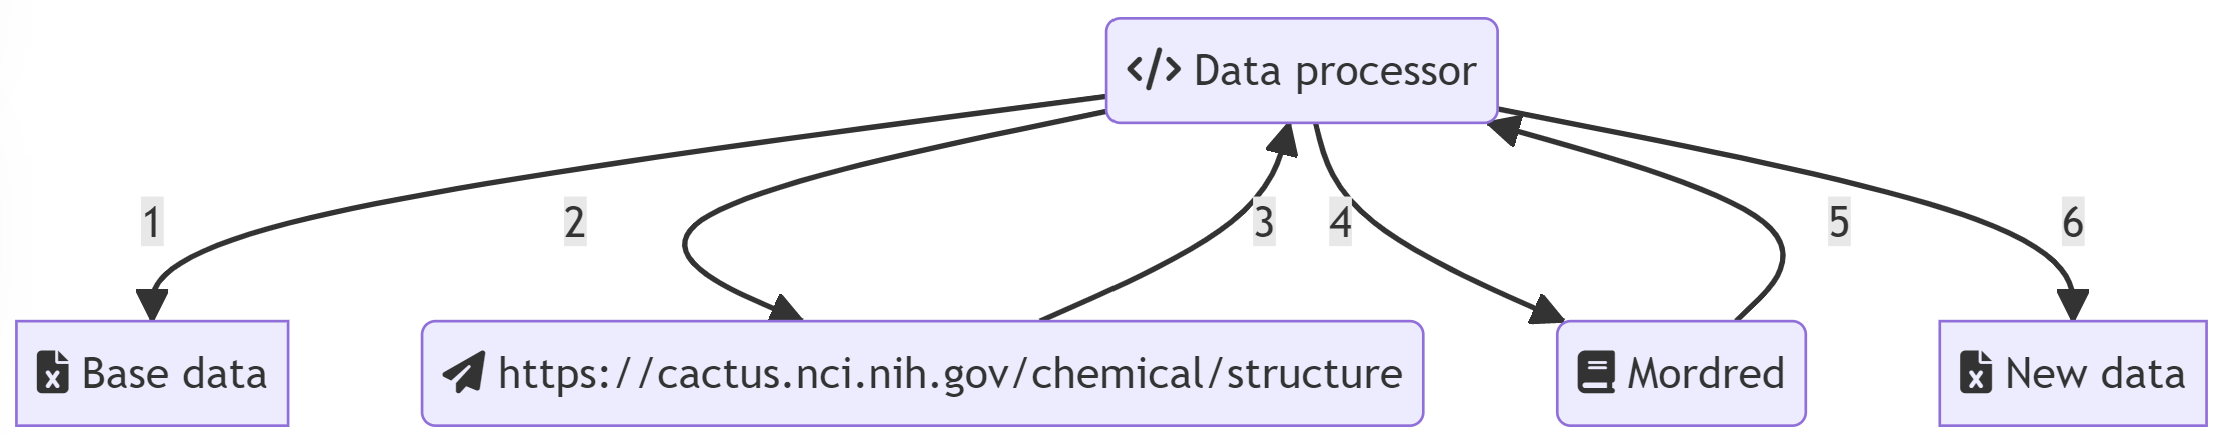
\includegraphics[width=140mm]{img/conception-data-construction.png}
    \captionof{figure}{Construction des données}
\end{center}

Le but est de prendre le nom des molécules depuis le fichiers excel existant et de traduire les noms en SMILES grâce à l'API de cactus.nci.nih.gov.
L'utilisation se fait simplement en faisant une requête HTTP GET sur l'URL suivante:
\begin{center}
    https://cactus.nci.nih.gov/chemical/structure/nomDeLaMolécule/smiles
\end{center}
Ensuite, il faut récrire les données dans un nouveau fichier excel.

Le temps de calcul des descripteurs est relativement long, il est donc intéressant de précalculer les descripteurs pour les liquides ioniques déjà présents dans le fichier excel.
Pour cela, il faut uitliser la libraire mordred\cite{mordred}.

La structure du fichier sera aussi modifiée pour faciliter la lecture des données par l'application.
Voici la structure du fichier excel de base:
\begin{itemize}
    \item IL structure: Informations des anions et cations utilisés (to test, Number, Abbreviation, Cation/Anion Full Name, Structure)
    \item Training set: Données pour l'entraînement du modèle (Cation, Anion, 99 features, Exp (K))
    \item Testing set: Données pour le test du modèle (Cation, Anion, 99 features, Exp(K))
\end{itemize}

La structure du fichier excel après la récolte des données sera:
\begin{itemize}
    \item IL structure: Informations des anions et cations utilisés (to test, Number, Abbreviation, Full Name et \acrshort{smiles})
    \item Training set: Données pour l'entraînement du modèle (\acrshort{smiles}, cation, anion et Exp (K))
    \item Testing set: Données pour le test du modèle (\acrshort{smiles}, cation, anion et Exp (K))
    \item Data descriptors: Descripteurs pré-calculés pour les liquides ioniques (\acrshort{smiles} du liquide, 900 features)
    \item Data old: Features du fichier de base (\acrshort{smiles} du liquide, 99 features)
\end{itemize}

Le fichier de base contient des feuilles qui ne sont pas détaillées ici mais elles ne sont pas utilisées dans ce projet.


% -----------------------------------------------------------------------------
\section{Pipeline de Machine Learning}
Comme pour la récolte des données, il faut aussi conceptualiser la pipeline de Machine Learning.
Dans ce cas, il y a deux use case.
Le premier est l'entraînement du modèle tandis que le second est la prédiction des données.

\begin{center}
    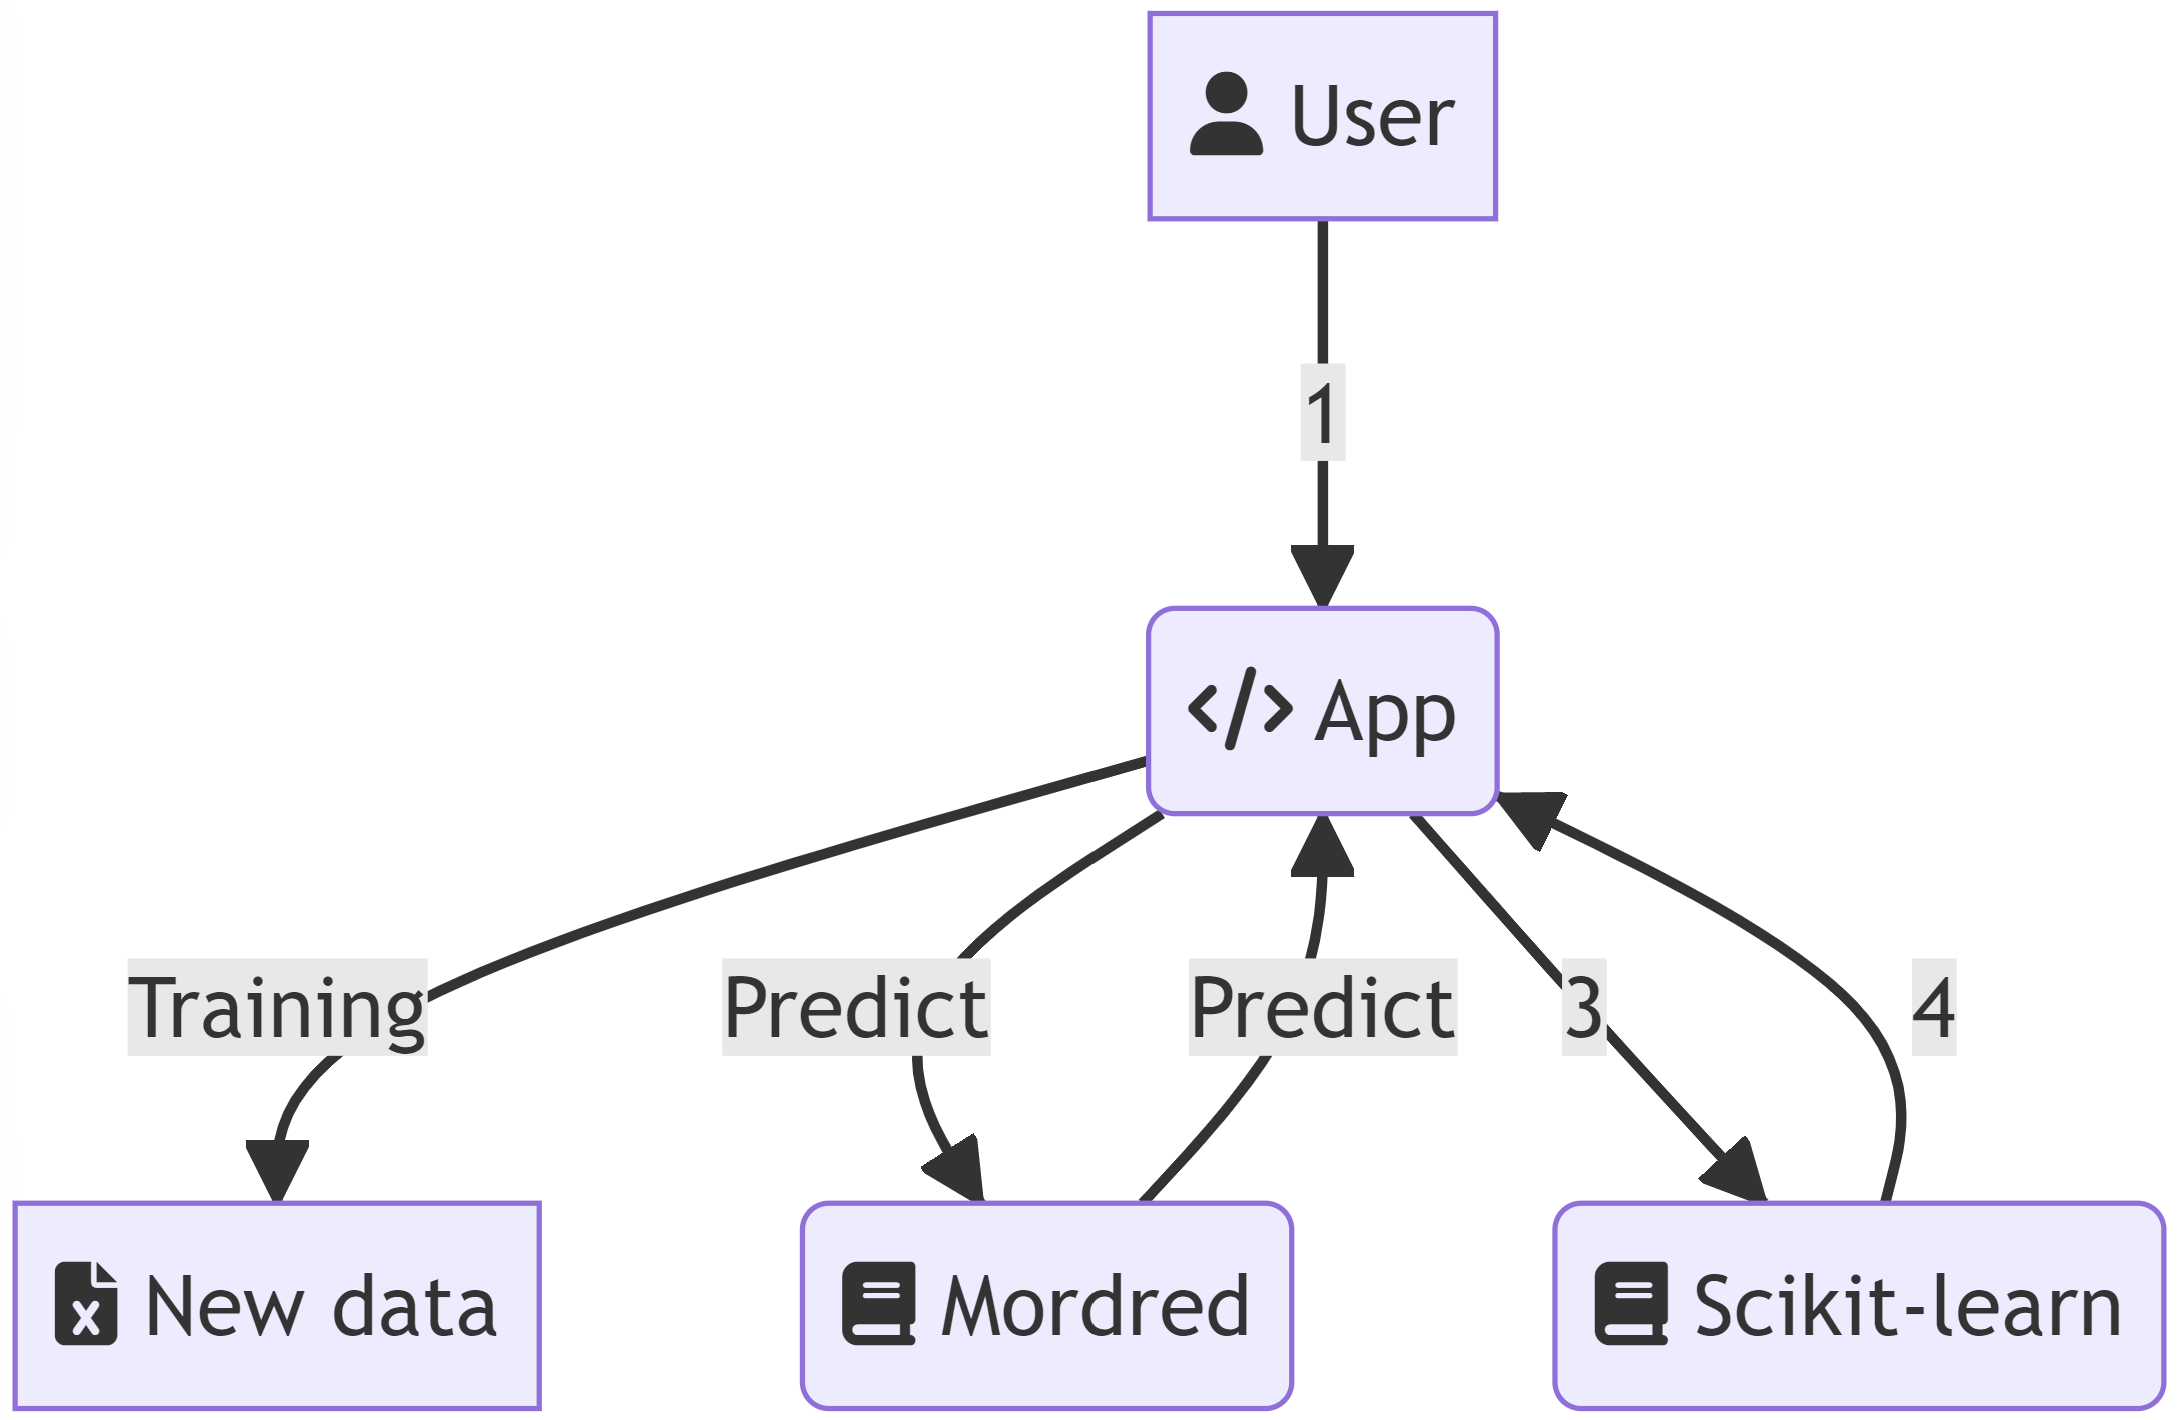
\includegraphics[width=100mm]{img/conception-ml-pipeline.png}
    \captionof{figure}{Activité de l'application de Machine Learning}
\end{center}

Le but est de fournir une seule application qui permet de tout faire et qui soit paramétrable à l'aide d'arguments.

% New page
\newpage
\subsection{Pipeline d'entraînement}
Si on rentre dans le détail de processus d'entraînement, il y a plusieurs étapes:
\begin{center}
    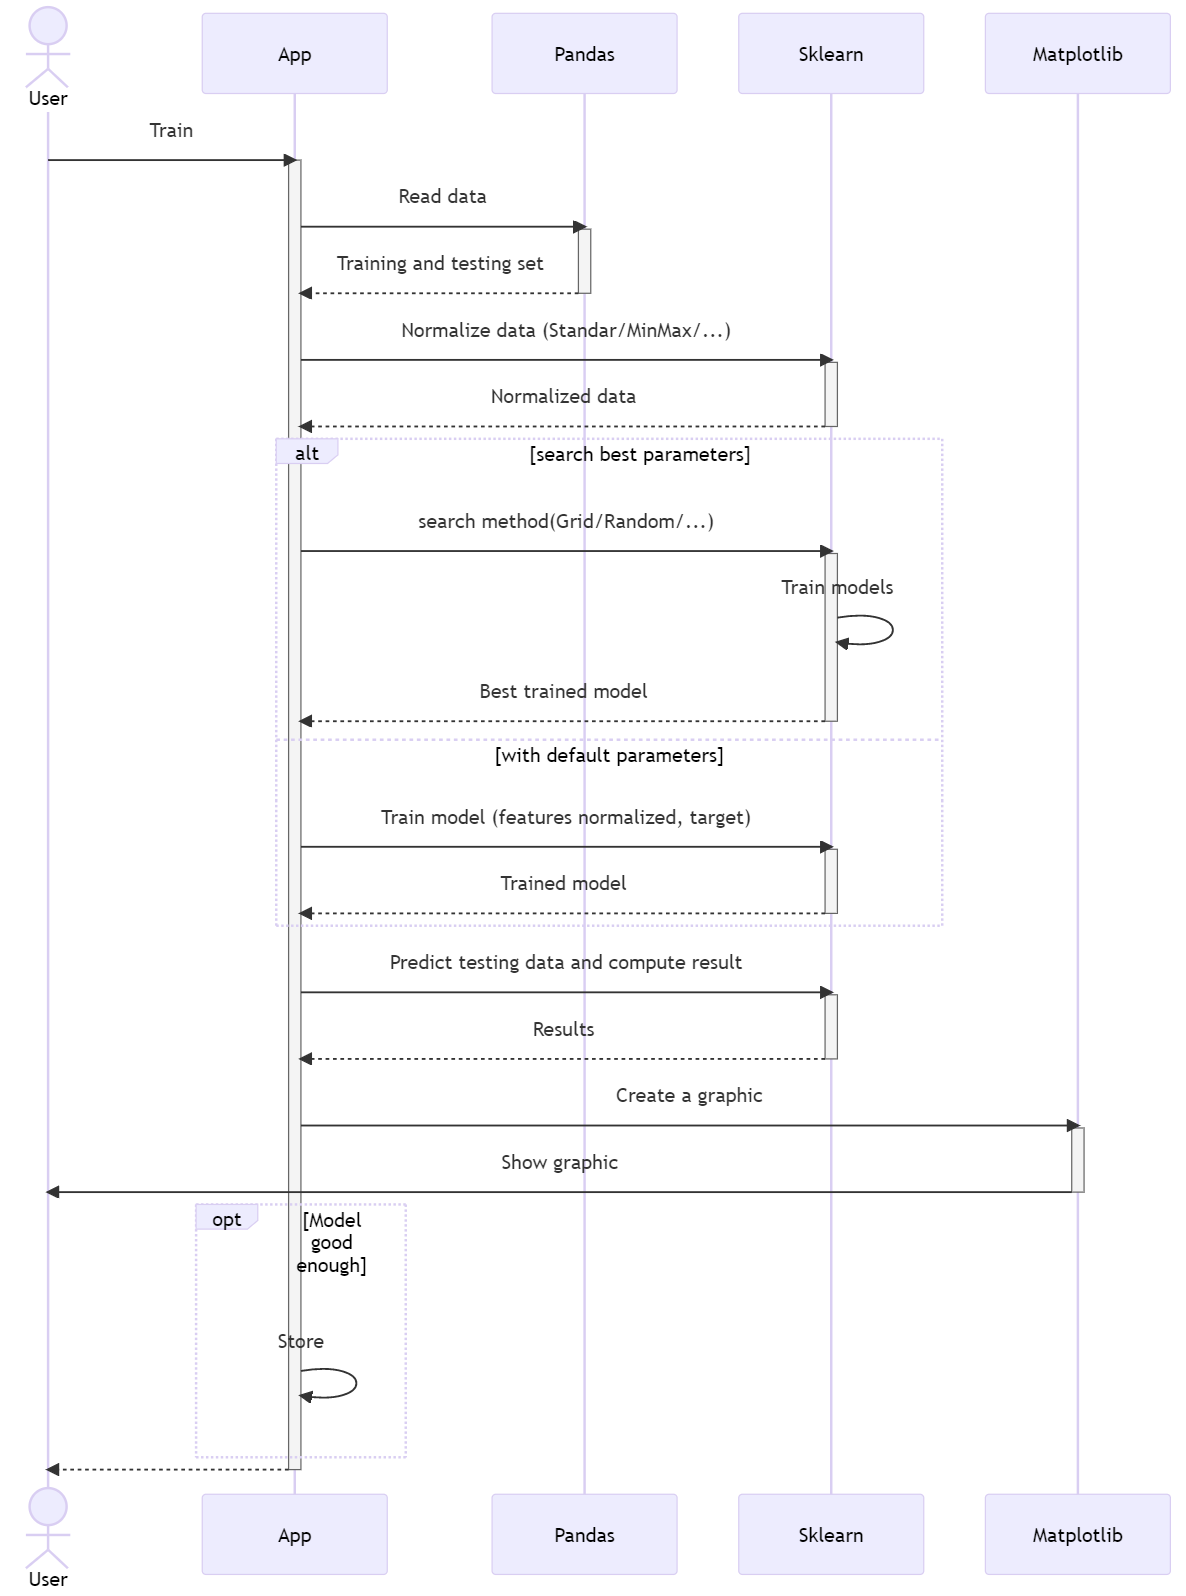
\includegraphics[width=140mm]{img/conception-ml-pipeline-training.png}
    \captionof{figure}{Pipeline de Machine Learning pour l'entraînement}
\end{center}

Le but est de pouvoir configurer chaque étape avec des paramètres lors du lancement du script.


\subsection{Sélection des features}
Pour sélectionner les bonnes features, il n'y a pas de méthode magique.
Ceci se fait par essaie-erreur en testant plusieurs combinaisons de features avec différents modèles et normalisation.
A cause du fait que le nombre de feature est important, il est difficile de les visualiser ou de les analyser.
Si les résultats sont plus mauvais qu'avec les donnnées de base, il faut essayer avec un mixte des données.
Si les modèles sont assez performants, ils sélectionnerons naturellement les bonnes features.
Si les meilleurs features ne sont que les features de base, ceci indique que les données rajoutées n'apportent rien d'utile à la prédiction.


%------------------------------------------------------------------------------
\section{Axe d'amélioration de l'\acrshort{ux}}
Si les résultats d'un modèle sont statisfaisant, il faudra ensuite le mettre à disposition de ChemTech pour qu'ils puissent l'utiliser.
Il y a 3 axes d'améliorations possible.

La premier est une version Desktop.
Je ne pense pas qu'il faut partir dans cette idée car l'utilisation est relativement simple et il y a le désanvatage de devoir l'installer.

La deuxième est un \acrfull{cli}.
Comme pour le version desktop, il y a le désanvantge de devoir l'installer, en revanche, ceci est beaucoup plus léger et cette solution est plus rapide à mettre en place.

La troisième est une version Web.
Cette solution n'a pas besoin d'être installée sur chaque ordinateur et l'application peut facilement être hébergé sur le serveur kubernetes de l'école.
Le désavantage est le temps de développement pour faire une vue et une \acrfull{api}.



\chapter{Implémentation}
\label{chap:implementation}
L'implémentation se fait dans deux fichiers python.
Le premier est\newline\texttt{fusion\_predictor.py}\cite{fusion_perdictor} qui permet de faire l'entraînement et l'analyse des données.
Le second est\newline\texttt{data\_processor.py}\cite{data_processor} qui permet de créer le nouveau fichier Excel à partir du fichier de Mme Yerly.
Ces deux fichiers s'utilisent avec des arguments qui permettent de choisir les étapes à effectuer et, si possible, de quelle manière.


% -----------------------------------------------------------------------------
\section{Récolte des données}
Le fichier python \texttt{data\_processo.py}\cite{data_processor} crée un nouveau fichier Excel à partir du fichier de Mme Yerly.
Il ajoute les \acrshort{smiles} et précalcule les descripteurs pour les liquides du fichier Excel.

Comme expliqué lors de la conception, le programme a plusieurs étapes et chacune de ces étapes sont optionnelles.
%show bash code
\begin{lstlisting}
python data_processor.py -h 
usage: data_processor.py [-h] [-t] [-r] [-d] [-a]

Create the new dataset.

optional arguments:
  -h, --help         show this help message and exit
  -t, --translate    Translate the name to smiles
  -r, --rewrite      Rewrite training set and test set
  -d, --descriptors  Compute the descriptors
  -a, --analyse      Analyse the dataset
\end{lstlisting}

Si un des paramètres est omis, le programme n'écrase pas les données dans le fichier Excel mais se contente de les lire.


% -----------------------------------------------------------------------------
\section{Analyse des données}
Pour analyser les données, il est possible d'utiliser le fichier \texttt{fusion\_predictor.py}\cite{fusion_perdictor} qui permet de générer de générer les rapports de pandas profiling.
Pour cela, il faut utiliser l'argument \texttt{analyse} en précisant \texttt{-o} ou non pour utiliser les données de bases.
Ces rapports sont utiles pour comprendre un peu mieux les features présentes et permet de trouver des correlation intéressantes.

% -----------------------------------------------------------------------------
\section{Entraîner un modèle}
Le script \texttt{fusion\_predictor.py} permet aussi d'entraîner un modèle.
Pour se faire il faut utiliser le paramètre \texttt{train} et plusieurs personnalisations sont disponibles
\begin{lstlisting}
python fusion_predictor.py -h
usage: fusion_predictor.py [-h] [--version]
                           [-o]
                           [-n {minmax,standard}]
                           [-b]
                           [-a {nusvr,svr,
                                randomforest,
                                gradientboosting}]
                           [-p {pca,kbest}]
                           [-s {random,grid}]
                           {analyse,train}

Find the fusion point of an ionic liquid.

positional arguments:
  {analyse,train}       Action to perform

optional arguments:
  -h, --help            show this help message and exit
  --version             show program's version number and exit
  -o, --old             Use the old data
  -n {minmax,standard}, --normalise {minmax,standard}
                        Normalise the data
  -b, --both            Normalise feature and target
  -a {nusvr,svr,randomforest,gradientboosting},
  --algorithm {nusvr,svr,randomforest,gradientboosting}
                        Algorithm to use
  -p {pca,kbest}, --preprocessing {pca,kbest}
                        Preprocessing to use
  -s {random,grid}, --search {random,grid}
                        Search algorithm to use
\end{lstlisting}

Les paramètres pour les rechreches doivent être écrit en dur dans le script.

\subsection{Sélection des données}
Comme nous avons deux set de données, il est possible de choisir lequel sera utilisé pour l'entraînement.
L'option \texttt{-o} permet d'indiquer que l'on veut utiliser les données de bases.


\subsection{Sélection des features}
Pour trier les features, il est possible d'utiliser de plusieurs méthodes.
Dans le script \texttt{fusion\_predictor.py}, cette étape s'appelle le preprocessing et elle est activable avec l'argument \texttt{-p}.

\subsection{Normalisation des données}
Pour normaliser les données, il est possible de faire de choisir entre deux méthodes.
La première est la normalisation \acrshort{minimax} utilisée par Mme Yerly et la seconde est la standardisation.
Ces options s'activent avec l'argument \texttt{-n} et la précision de l'algorithme voulu.

\subsection{Sélection du modèle}
Comme pour les deux étapes précédentes, il est possible de choisir entre plusieurs algorithmes.
Ce choix se fait avec l'argument \texttt{-a} et la précision de l'algorithme voulu.
Ceci prendra les hyper paramètres par défaut de la librairie \acrshort{sklearn}.
Il est possible de faire rechercher les meilleurs hyper paramètres avec l'argument \texttt{-s} qui activera un \texttt{grid\_search} ou un \texttt{random\_search}.
Les paramètres de recherche doivent être écrit en dur dans le fichier \texttt{fusion\_predictor.py}.

% -----------------------------------------------------------------------------
\section{Amélioration de l'\acrshort{ux}}
Par manque de temps et de résultats satisfaisants, cet aspect n'a pas été traité mais la solution préconisée est celle d'une application web.

\chapter{Résultats}
\label{chap:Résultats}

Dans l'ensemble, les résultats sont plutôt décevants.
En effet, les modèles n'ont pas réussi à prédire les résultats avec de meilleure performance que le modèle de base.
Cependant, il est possible de tirer quelques enseignements de ces résultats comme le fait que \acrshort{svm} n'est pas fait pour les larges set de données ou que la normalisation n'est pas forcément un facteur important.


% -----------------------------------------------------------------------------
\section{Récoltes des données}

Tous les noms de molécules ne sont pas traductible en \acrshort{smiles}.
De plus, la librairie mordred n'arrive pas à calculer les descripteurs pour toutes les molécules.
C'est pourquoi, nous avons quelques pertes sur les nouvelles données.
Le nombre de liquides ioniques était de 765 et il est passé à 739 ce qui nous fait une perte de 3,4\%.
Si on regarde l'implication sur les datasets, nous avons le training set qui passe de 600 à 583 et le test set qui passe de 168 à 159.
Ceci fait respectivement une baisse de 2,8\% et 5,4\%.
Les données ont déjà été complétée à la main par Chemtech.

% -----------------------------------------------------------------------------
\newpage
\section{Choix des modèles}
En prenant les nouvelles données non normalisées et en utilisant les paramètres par défaut des modèles, nous pouvons nous faire une idée de la performance de chacun et des résultats qu'ils donnent.

\begin{figure}[ht]
    \centering
    \subfloat[\centering \acrshort{nusvr} avec les paramètres de Mme Yerly]{{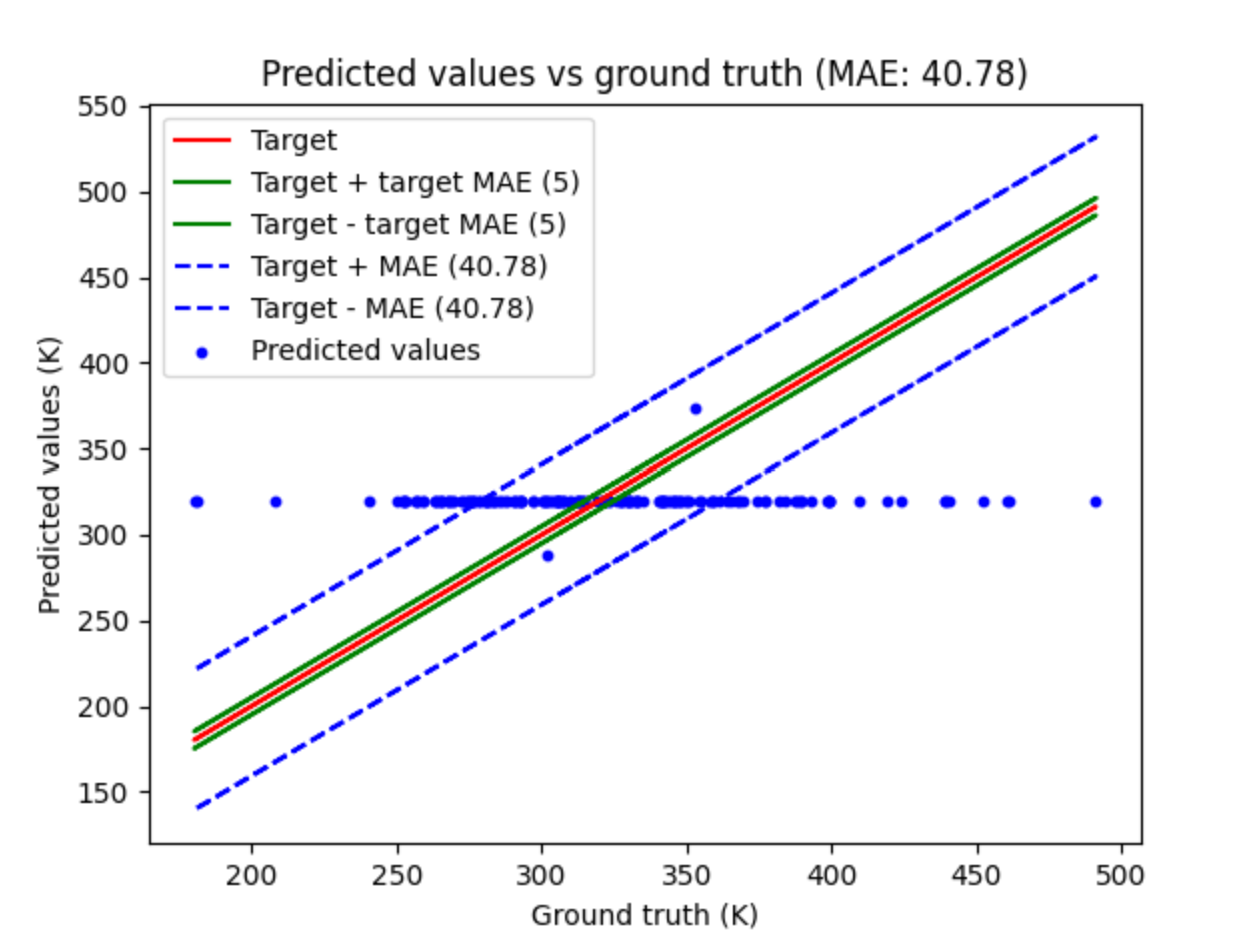
\includegraphics[width=60mm]{img/result_nusvr_noNorm.png}}}
    \qquad
    \subfloat[\centering \acrshort{svm}]{{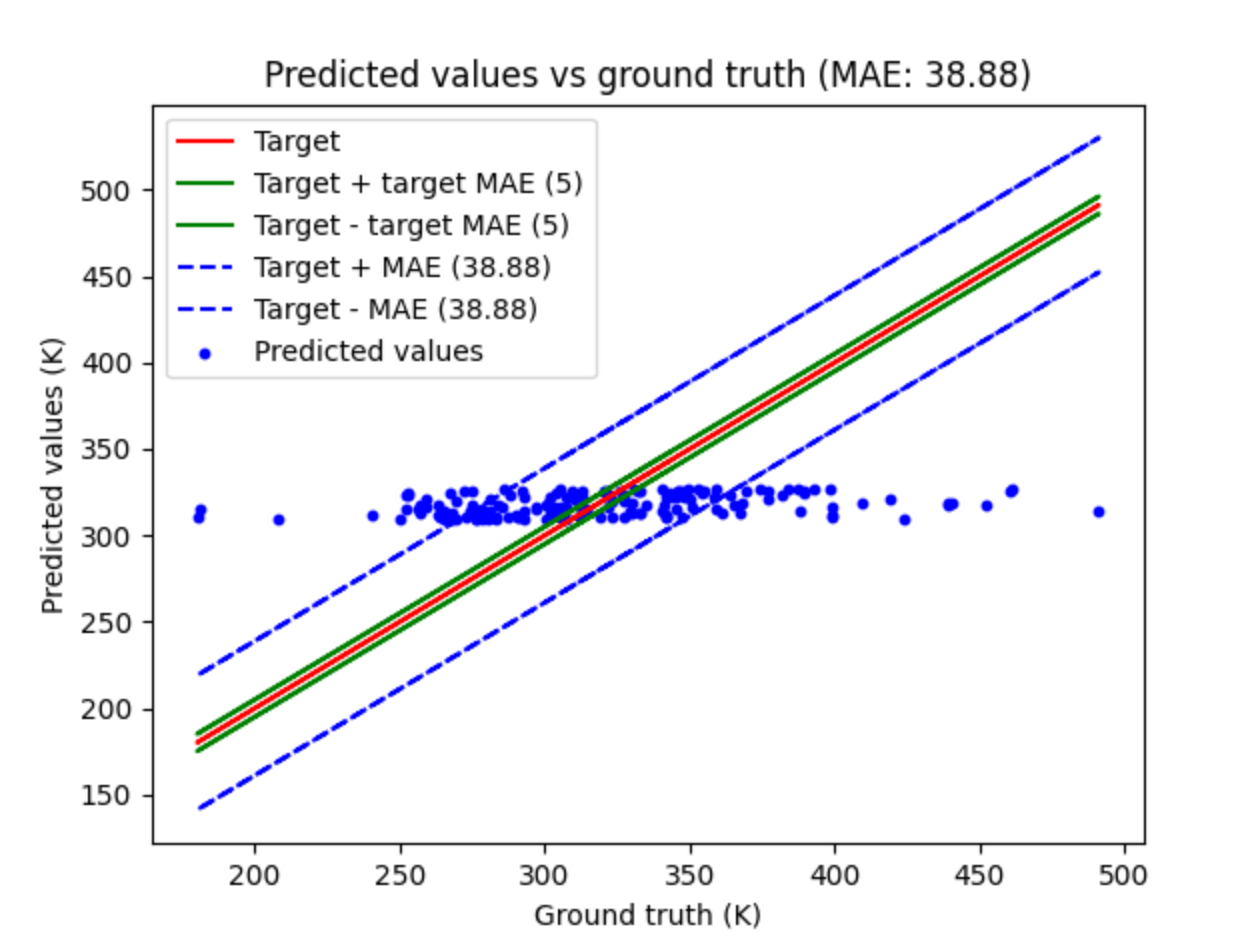
\includegraphics[width=60mm]{img/result_svr_noNorm.png}}}
    \qquad
    \subfloat[\centering Random forest]{{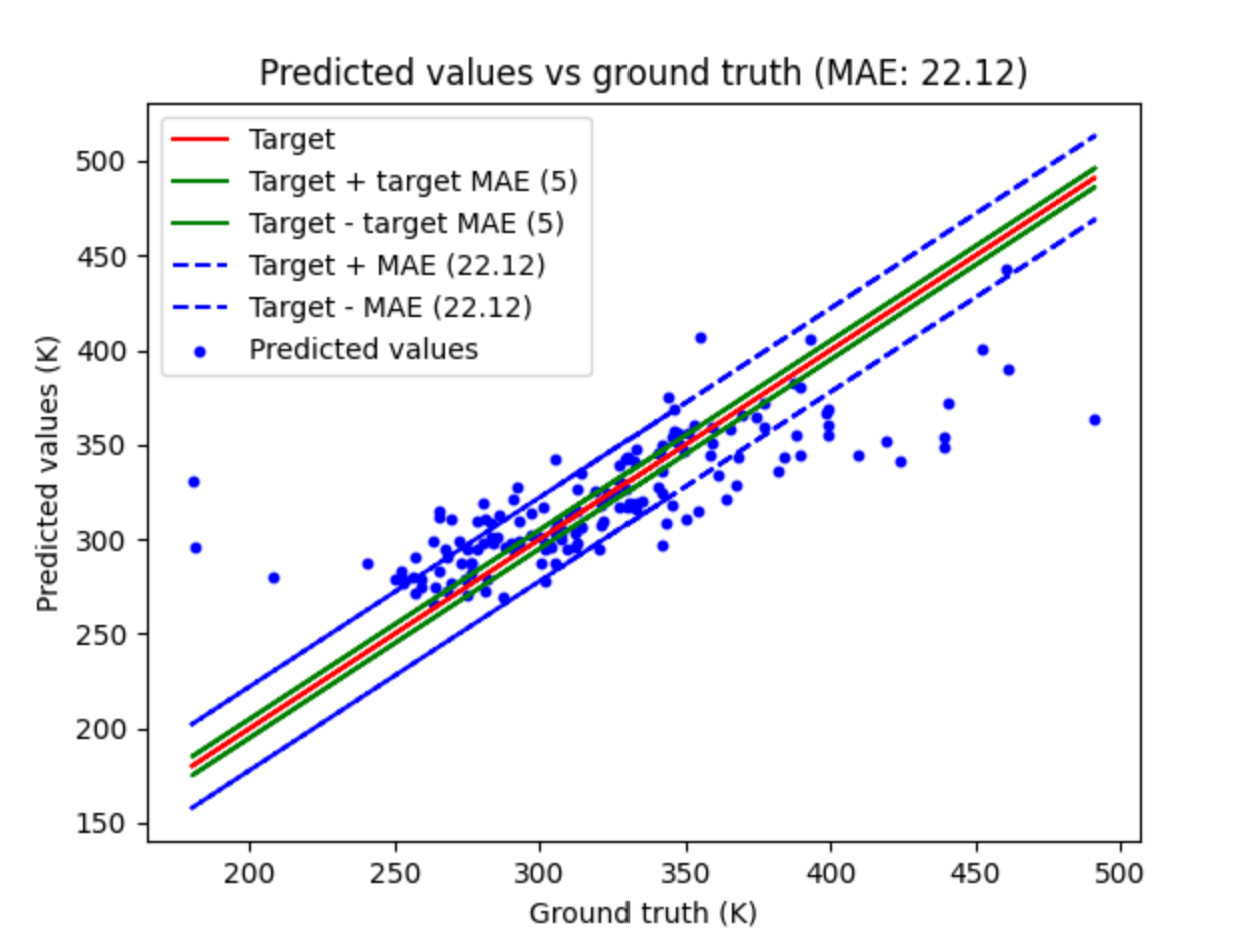
\includegraphics[width=60mm]{img/result_rf_noNorm.png}}}
    \qquad
    \subfloat[\centering Gradient boosting]{{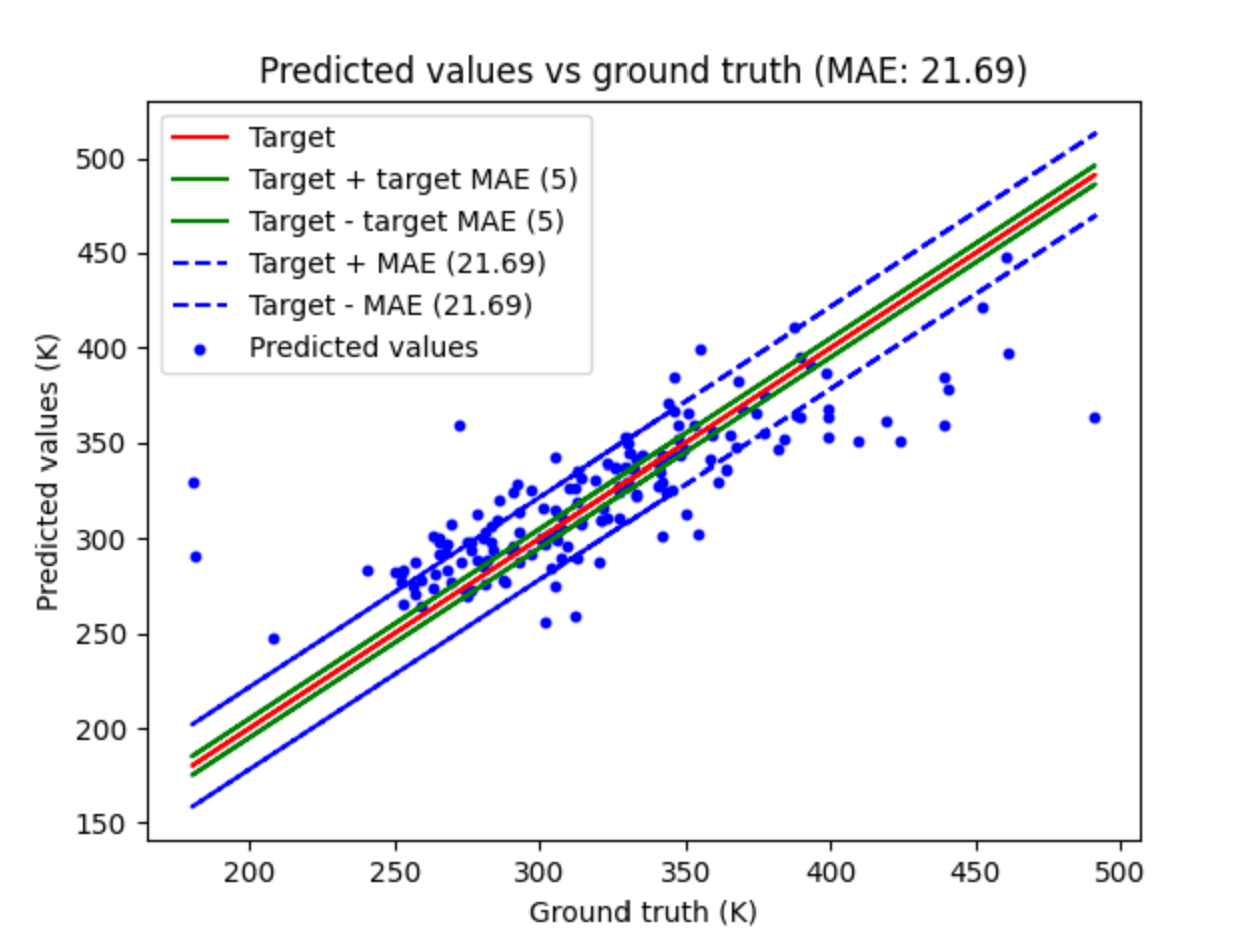
\includegraphics[width=60mm]{img/result_gb_noNorm.png}}}
    \captionof{figure}{Résultats des modèles avec les paramètre par défaut sans normalisation ni preprocessing}
\end{figure}

Ce qui ressort c'est que \acrshort{svm} n'est pas performant avec un large set de données.
Ce qui est flagrant c'est la difficulté qu'ont les modèles à prédire les données et ils font un compromis pour mettre toutes les données dans la moyenne.


\newpage
\subsection{Normalisation}
Les résultats étant très mauvais sur les \acrshort{svm}, ils seront écartés de la suite des expériences.
La normalisation est un facteur important dans la modèle de régression.

\begin{figure}[ht]
    \centering
    \subfloat[\centering Random forest normalisé avec \acrshort{minimax}]{{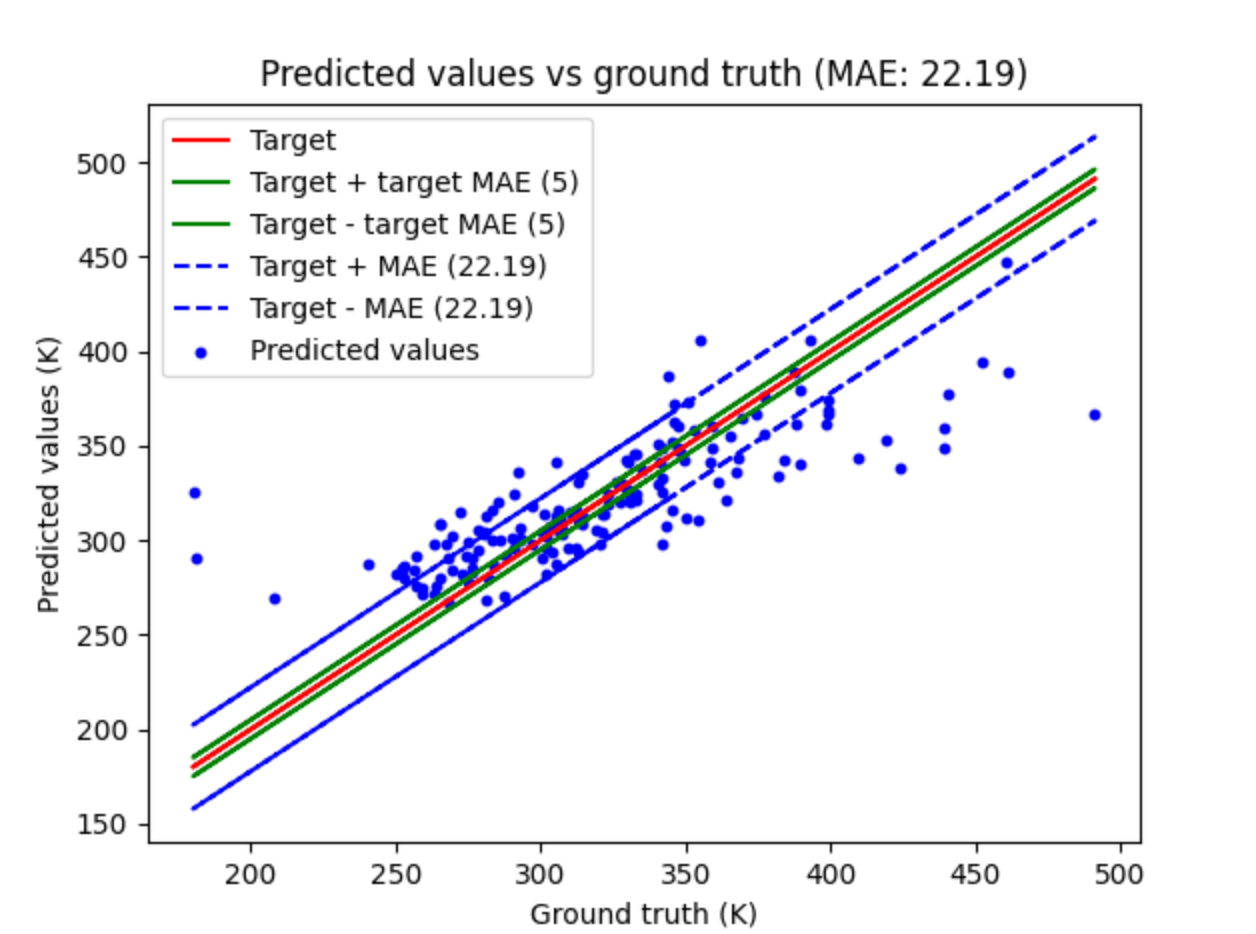
\includegraphics[width=60mm]{img/result_rf_minmax.png}}}
    \qquad
    \subfloat[\centering Gradient boosting normalisé avec \acrshort{minimax}]{{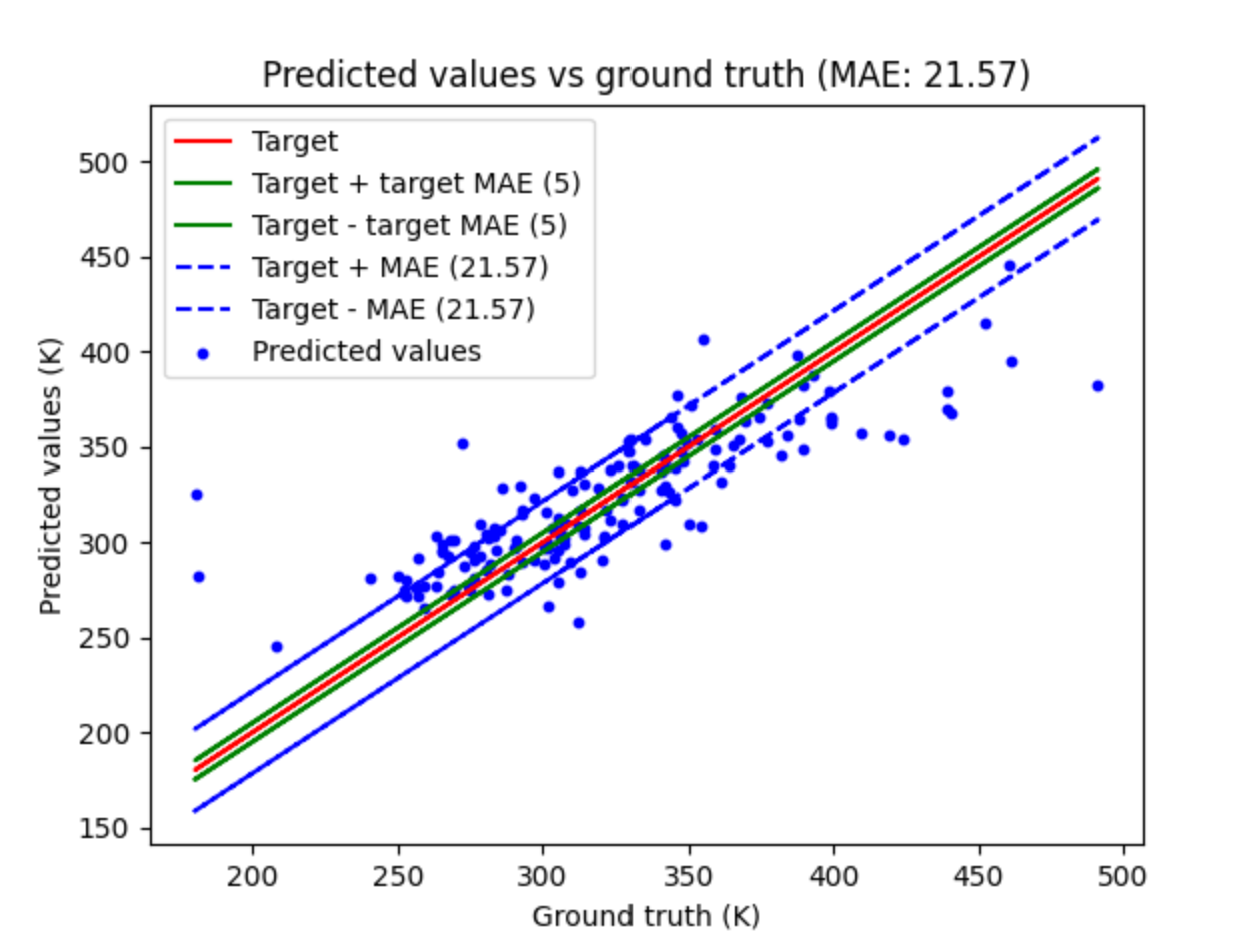
\includegraphics[width=60mm]{img/result_gb_minmax.png}}}
    \qquad
    \subfloat[\centering Random forest standardizé]{{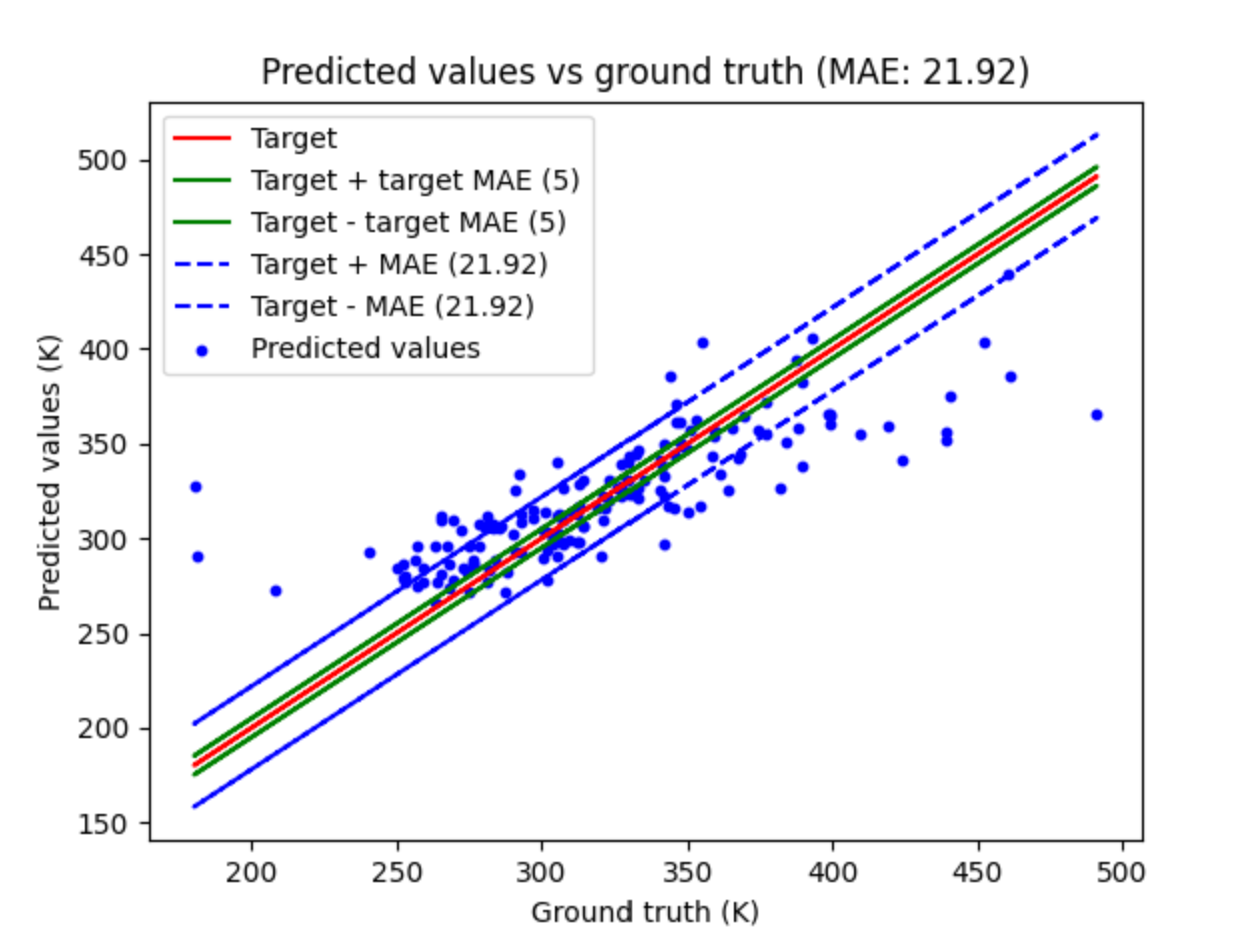
\includegraphics[width=60mm]{img/result_rf_standard.png}}}
    \qquad
    \subfloat[\centering Gradient boosting standardizé]{{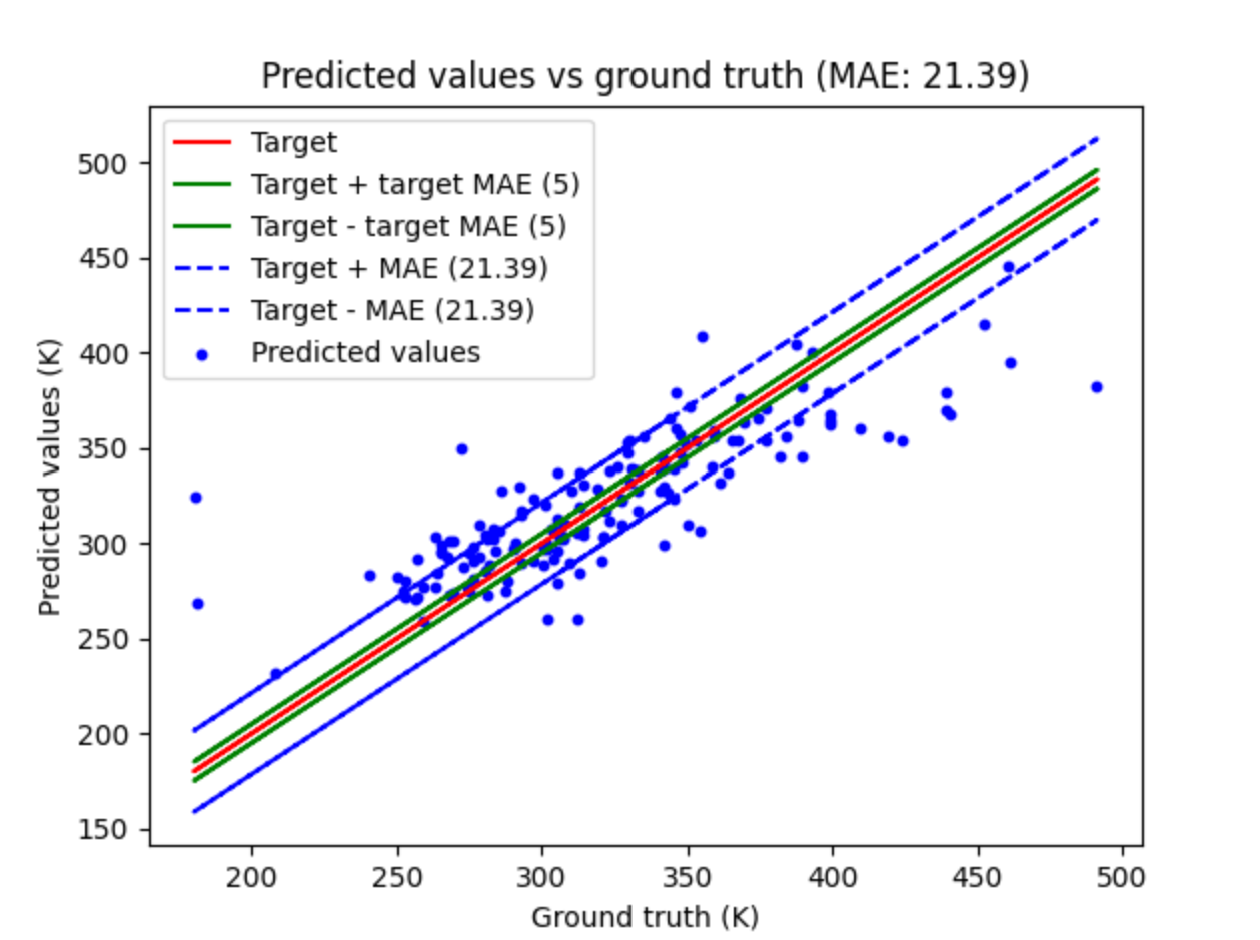
\includegraphics[width=60mm]{img/result_gb_standard.png}}} 
    \captionof{figure}{Résultats des modèles avec les paramètre par défaut et différente normalisation}
\end{figure}

Les résultats ne s'améliorent pas significatievement avec la normalisation.

\subsection{Autres axes}
D'autre axes d'améliorations ont été explorer comme le \acrfull{pca} mais les résultats étaient similaires.
Une hypothèse intéressante était de fusionner les nouvelles données avec les données de Mme Yerly et de voir si les modèles obtenaient les mêmes résultats que lors de la reproduction.
Si cette s'étaiet vérifié, cela aurait indiqué que les nouvelles données n'apportaient rien de plus.
Malheureusement, les résultats n'étaient pas mieux mais les features sélectionnées faisaient partie des deux jeux de données.



\chapter{Conclusion}
\label{chap:conclusion}
Ce projet est typiquement le genre de projets qui peuvent ne jamais avoir de fin.
En effet, l'\acrshort{eda} peut durer des mois et les améliorations de modèles sont quasiment infinies.
Ce projet étant un projet de semestre 5 nous ne disposons pas de temps illimités.

% -----------------------------------------------------------------------------
\section{Résumé du projet}
Pour résumer ce projet, il s'agit du développement d'un modèle de machine learning capable de prédire la température de fusion d'un liquide ionique avec une précision de 5° Kelvin.
Le projet a été bâtis sur un précédent projet au sein de la \acrshort{heia-fr} et avait pour but de battre les performances du modèle de base.

Les activités étaient découpées en 3 parties.
La première consistait à reproduire les résultats du modèle de base.
Ceci a été fait avec le nouveau fichier Excel et la librairie \acrshort{sklearn}.
La deuxième partie était la création d'un nouveau fichier Excel contenant les mêmes dataset que la première version tout en ajoutant les descripteurs.
Cette étape est nécessaire pour la création du nouveau modèle et est probablement la plus grosse plus-value de ce projet.
En effet, dans le cas où le nouveau modèle n'est pas meilleur que celui de base, les données pourront toujours être reprises et tester avec d'autres modèles.
La troisième et dernière partie, consistait à créer un nouveau modèle de machine learning utilisant les données obtenues avec les descripteurs.
Cette étape n'a pas portée ses fruits et aucun modèle n'a été capable de battre significatievement le modèle de base et encore moins de se rapprocher de la précision de 5° Kelvin.


% -----------------------------------------------------------------------------
\section{Problèmes rencontrés}
Le projet s'est déroulé sans problème majeur. A part le dernier objectif qui n'a pas été atteint, le projet a été mené à bien.
Cet échec s'explique par le fait que je suis débutant dans le domaine du \acrlong{ml}.
J'ai trouvé que ce domaine est très vaste et demande une certaine expérience afin de pouvoir créer des modèles performants.

% -----------------------------------------------------------------------------
\section{Axes d'améliorations}
Le projet possède deux grands axes d'améliorations. Le premier est au niveau de la performance et le second se concentre plus sur l'\acrlong{ux}.

Les performances des modèles étant décevantes, il est naturelle de penser qu'il est possible d'en développer de meilleurs.
Ceci passera par une \acrlong{eda} plus poussée et des connaissances en chimie afin de préselectionner les features intéressantes.

Du point de vu de l'\acrshort{ux}, le projet est livré avec deux fichiers\cite{data_processor}\cite{fusion_perdictor} python s'utilisant avec des paramètres. 
Il serait très intéressant de développer une version web qui permettrait de faire des prédictions sans avoir à installer des librairies python.
Ceci aurait aussi l'avantage d'avoir une interface graphique plus agréable.

% -----------------------------------------------------------------------------
\section{Avis personnel}
Personnellement, j'ai trouvé ce projet très intéressant et enrichissant.

Tout d'abord, j'ai exploré le monde de la chimie qui est un domaine que je ne connaissais que très peu mais il m'intéresse car j'ai beaucoup de connaissances dont c'est leur métier.
Ensuite, j'ai fait ce projet de \acrlong{ml} en même temps que le cours. Ceci n'a pas été facile car la théorie et la pratique étaient assez souvent dissociées.
En effet, les thèmes n'étant pas forcément synchronisés, j'ai beaucoup tatônner dans ce projet.
Malgré ces contre-temps, je ne regrette pas du tout mon choix et je suis très content de l'avoir fait.

En ce qui me concerne, j'estime avoir eu une bonne gestion de projet avec l'utilisation, au maximum, de GitLab.
J'ai trouvé que la documentation en LaTex avec une pipeline était très pratique pour partager mon avancée.
Par contre, la gestion du planning est à revoir car les outils ne sont pas très pratiques à utiliser.
J'ai aussi apprécié le fait de devoir faire une mini-présentation à chaque weekly-meeting.
Ceci me permettait d'avoir un fil rouge tout au long des séances et facilitait la rédaction de mes PVs.
En revanche, je déplore mon manque de rigueur sur la tenue de la documentation et du maintien de mon code que j'ai dû rattraper à la fin du projet.

\chapter{Déclaration sur l'honneur}
\label{chap:honneur}
Je, soussigné, Simon Barras, déclare sur l'honneur que le travail rendu est le fruit d'un travail
personnel. Je certifie ne pas avoir eu recours au plagiat ou à toutes autres formes de fraudes.
Toutes les sources d'information utilisées et les citations d'auteur ont été clairement mentionnées.

\chapter{Remerciements}
\label{chap:remerciement}
Je tiens à Remercier M Wolf et son assistant M Donzallaz pour leur aide et leur disponibilité.
Ils m'ont aiguillé de nombreuses fois et m'ont permis de m'améliorer dans le domaine du \acrlong{ml}.
Je souhaite aussi remercier Mme Yerly qui a réalisé les bases du projets et m'a aidé de nombreuses fois à comprendre les données.
Pour finir, je remercie M Marti et son institut ChemTech pour la confiance accordé et pour la complétion et validation des données chimiques que je n'aurais en aucun cas pu faire moi-même.
J'apporte une mention spéciale à Github Copilot pour m'avoir aidé à écrire ce rapport et Simon Braillard pour la relecture du rapport.

\chapter{Logiciels utilisés}
\label{chap:logiciel}
Voici la version de pyhton ainsi que les librairies utilisées pour ce projet.

\begin{table}[ht]
    \centering
    \begin{tabular}{|l|l|}
    \hline
    \multicolumn{1}{|c|}{\textbf{Logiciel}} & \multicolumn{1}{c|}{\textbf{Version}} \\ \hline
    Python                                  & \multicolumn{1}{c|}{3.9.15}           \\ \hline
    aiohttp                                 & \multicolumn{1}{c|}{3.8.3}            \\ \hline
    matplotlib                              & \multicolumn{1}{c|}{3.6.3}            \\ \hline
    mordred                                 & 1.2.0                                 \\ \hline
    numpy                                   & 1.23.4                                \\ \hline
    openyxl                                 & 3.0.10                                \\ \hline
    pandas                                  & 1.5.1                                 \\ \hline
    pandas-profiling                        & 3.6.2                                 \\ \hline
    rdkit                                   & 2022.9.2                              \\ \hline
    scikit-learn                            & 1.1.3                                 \\ \hline
    \end{tabular}
    \captionof{table}{Logiciels utilisés pour ce projet}
\end{table}




% Appendices
% \appendix

% -----------------------------------------------------------------------------
% Back matter
% -----------------------------------------------------------------------------
% \backmatter

% List of figures
%\cleardoublepage
\phantomsection
\addcontentsline{toc}{chapter}{Table des figures}
\listoffigures
\addcontentsline{toc}{chapter}{Table des tableaux}
\listoftables

% Bibliography
%\cleardoublepage
\printbibliography[title={Références}, heading=bibintoc]

% Glossary
\glsaddall
\printglossary[type=\acronymtype, nonumberlist]
% TODO: Add index

% Add your CV here if you want

\end{document}

